\documentclass{homework}

\title{Micropropulsion \\ Individual Assignment}
\author{Ulf Torsten Kemmsies - 4794281  \\
MSc. Space Engineering - TU Delft}
\usepackage{geometry}
\usepackage{graphicx}
\graphicspath{ {./images/} }
\usepackage{amsmath}
\usepackage[table,xcdraw]{xcolor}
\usepackage{lscape}
\usepackage{multicol} % For multiple columns
\usepackage{capt-of} % For creating captions outside of floats

\begin{document}

\maketitle

\begin{abstract}
    This paper presents a novel approach to designing vaporizing liquid micropropulsion systems, vital for precise small satellite control. By integrating analytical models and characterizing flow behavior, the study addresses fluid dynamics, heat transfer, and combustion complexities. The approach employs comprehensive simulation, Latin Hypercube Sampling, and optimization to explore the parameter space, revealing optimal designs and sensitivities. Despite challenges, this integrated framework enhances efficiency and reliability of future micropropulsion systems for small satellite missions. Results highlight improved thrust and specific impulse efficiencies, reduced mass flow errors, and minimized heating power.
\end{abstract}

\begin{center}
Github repository: \url{https://github.com/ulfkemmsies/micropropulsion-VLM-design}    
\end{center}

\begin{multicols}{2} % Start two-column layout
\section{Introduction}

This paper presents a comprehensive approach to designing the next generation of vaporizing liquid micropropulsion systems by combining existing analytical models and characterizing the flow behavior. Micropropulsion systems play a crucial role in various space missions, enabling precise control and maneuverability of small satellites. However, the design and optimization of these systems remain challenging due to the complex interplay of fluid dynamics, heat transfer, and combustion processes.

TU Delft has been one of the centers of research around Vaporizing Liquid Microthrusters, with several papers published in the past few years considering different aspects of VLMs.

However, each model depends on assumptions that limit its predictive power experimentally, and often focus on single elements of the VLM, like the flow in the heating chamber microchannels, the nozzle's performance, or control of the propellant injector to ensure constant thrust. There is a gap in the literature for an integrated model which characterizes the entire VLM's behavior based on a few inputs, mainly related to sizing the system.

To address these challenges, this study proposes a novel framework that integrates multiple analytical models to enhance the understanding and performance of vaporizing liquid micropropulsion systems. By leveraging existing models, we aim to capitalize on their strengths and overcome their limitations, ultimately leading to more accurate predictions and efficient designs.

The first step involves a comprehensive review and selection of relevant analytical models for key components of the micropropulsion system, including combustion chamber and nozzle.

Each model is carefully evaluated based on its applicability, accuracy, and computational efficiency. Subsequently, these models are integrated into a unified framework, allowing for a holistic analysis of the system's behavior.

By combining existing analytical models and characterizing flow behavior, we can overcome the limitations of individual models and achieve a more comprehensive understanding of system performance. This, in turn, will facilitate the design of next-generation micropropulsion systems that offer enhanced efficiency, reliability, and maneuverability for small satellites in space missions.

\section{Literature Review and Modeling}

The given source material was composed of previous student-led investigations on the topic and professional research by TUD researchers.

\subsection{Model overview}

\begin{minipage}{\linewidth}
      \centering
      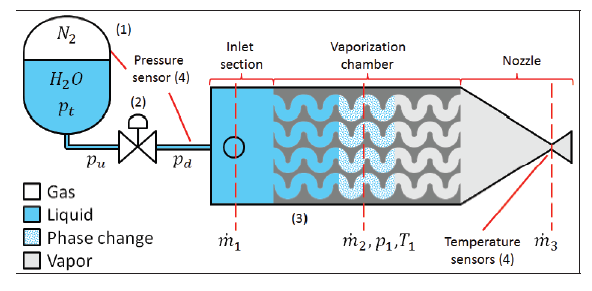
\includegraphics[width=\linewidth]{images/overview.png}
      \captionof{figure}{General Physical VLM Model}
      \label{fig:model_overview}
  \end{minipage} 

The general structure of the VLM is taken from \cite{silva_comprehensive_2019} and is shown in Figure \ref{fig:model_overview}. Water is pressurized to mimic the conditions of a blow-down propellant feed and fed into the inlet of the heating chamber. A resistive heater is used to heat the walls of the microchannels of the chamber.g. The resulting vapor is accelerated through the remaining channel length toward the micronozzle. The nozzle is a standard axisymmetric choked convergent-divergent type.


The assumptions for the system under consideration are as follows:

\begin{enumerate}
    \item Water enters the system at the inlet under pressure and at a standard temperature of 22°C. The corresponding density of the water is 997.8 kg/m3.
    
    \item There is no liquid pressure loss from the tank to the inlet, and from the inlet until boiling. This is due to the very small magnitude of losses relative to operational pressures.
    
    \item The vaporized propellant is further heated in the chamber, but no further significant heat transfer between the wall and gas occurs in the nozzle. The flow speed in the chamber is negligible relative to the that in the nozzle, and as such, the conditions at the end of the chamber are treated as the stagnation condition.
    
    \item The nozzle is assumed to have axisymmetric choked flow, meaning that the throat flow is sonic and therefore the relevant equations can be used.
    
    \item The heating power is uniformly distributed over the heated surface area in the heating chamber (i.e. uniform heat flux). The system uniformly heats the entire volume of liquid and vapor mixture, and all the walls of the heating chamber and nozzle are at the same temperature, denoted as $T_w$.
    
\end{enumerate}

\subsection{General Equations}

\subsubsection{Ideal Gas Relation}
	    
	  The ideal gas theory is a simplified model that describes the behavior of gases under certain conditions. It assumes that gas particles are point masses with no volume, and that they move randomly and independently. The theory states that the pressure, density, and temperature of an ideal gas are related by the equation:  
	    
	  $$ P = \rho \cdot R_s \cdot T $$  
	    
	  where $P$ is the pressure, $\rho$ is the density, $R_s$ is the ideal gas constant, and $T$ is the temperature in Kelvin.  
	    
	  It is important to note that this theory assumes incompressibility, and therefore cannot be used once the Mach number $ Ma > 0.3$ , which means anywhere in the nozzle, since choked flow at the throat is assumed. If the real gas behavior were to be modelled fully, the relation

        $$P v= Z \cdot \rho \cdot R_s \cdot T$$ 

        would need to be used, with $Z$ being a compressibility factor established experimentally. However, at "low" pressures, meaning anything below 10 bar, the compressibility factor is very close to one, and thus the ideal gas relation can be used unchanged. \cite{Libretexts_2022}
        
\subsubsection{Speed of sound}
	    
	  The speed of sound refers to the rate at which sound waves propagate through a medium. It is influenced by various factors, including the properties of the medium and the temperature. In an ideal gas, the speed of sound can be determined using the equation:  
	    
	  $$
	  a = \sqrt{\gamma \cdot R \cdot T}
	  $$  
	    
	  where
	  $a$ represents the speed of sound,  
	  $\gamma$ denotes the adiabatic index (also known as the heat capacity ratio),  
	  $R$ represents the specific gas constant, and  
	  $T$ denotes the temperature of the medium.  
	    
	  It is important to note that this equation assumes an ideal gas behavior and neglects other factors that may affect the speed of sound, such as humidity or pressure.  
\subsubsection{Kinematic viscosity}
	    
	  Kinematic viscosity is a measure of a fluid's resistance to flow under the influence of gravity. It is defined as the ratio of dynamic viscosity to density. The equation for kinematic viscosity ( $\nu$ ) is given by:  
	    
	  $$\nu = \frac{\mu}{\rho}$$  
	    
	  where $\mu$ represents the dynamic viscosity and $\rho$ represents the density of the fluid.  
\subsection{Sizing}

\subsubsection{Heating Chamber}
	  This chamber consists of wavy microchannels with 3 heated sides (the top wall consists of the next layer in the assembly) and a fixed geometry taken from \cite{bianchi_micropropulsion_nodate} as shown in Figure \ref{fig:element_dimensions}. In order to simplify the modeling process, the standard unit was used unaltered, and this geometry is repeated $n_{elem}$ times along the length of the chamber to form a single channel. Along the width of the VLM, $n_{chan}$ channels are used to form the complete heating chamber.

   \begin{minipage}{\linewidth}
      \centering
      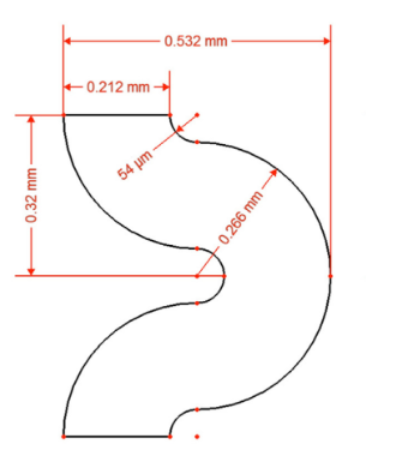
\includegraphics[width=\linewidth]{images/image_1691249918616_0.png}
      \captionof{figure}{Dimensions and geometry of single heating chamber element}
      \label{fig:element_dimensions}
  \end{minipage} 
	    
	  The centerline $L_C = 1.00714$ mm and length $L = 0.64$ mm of one such element have been previously determined, and need only be multiplied by the number of elements to be calculated for the whole chamber.  
	    
	  The other main sizing variable for the heating chamber is the chamber depth $H$ , which will determine the total area of the heated walls $A_{heat}$ when multiplied by the integrated wall length according to $$(2.01062 \ mm \cdot H + 0.213126 \ mm^{2} ) \cdot n_{elem} \cdot n_{chan}$$ The total volume of the chamber $V_{tot}$ is similarly calculated using $$ (0.213126 \ mm^{2} \cdot H ) \cdot n_{elem} \cdot n_{chan}$$  
	    
	  Finally, the hydraulic diameter of this same cross-section is calculated with $$D_h=\frac{4 A}{p}$$ where $A$ is the cross-sectional area and $p$ the rectangular perimeter.  
   
\subsubsection{Nozzle}
	  The micronozzle has three main sizing input variables: the throat radius $R_t$ , the exit radius $R_e$ and the nozzle length $L_n$. The diverging section of the nozzle is assumed to expand outward from the throat without any curvature, so that the length along the nozzle wall can be found with $$ x = \sqrt{R_{e}^2 + L_{n}^2} $$ and the nozzle exit half-angle with $$ \alpha = \tan^{-1} \left( \frac{R_{e}}{L_n} \right) $$
   
\subsection{Heating Chamber Liquid Phase}

The assumptions of the model used in this phase, in the original paper \cite{bianchi_micropropulsion_nodate}, are as follows:
\begin{itemize}
    \item Incompressible flow
    \item Steady state (this was verified with transient simulations)
    \item Negligible radiative and natural convective heat transfer
    \item Negligible viscous dissipation
    \item Laminar flow
    \item Constant fluid properties
\end{itemize}

	  This is due to the extremely low Reynolds numbers found in that investigation, and in order to keep the validity of the model intact, we must design our liquid flow phase according to those low Reynolds numbers. Additionally, constant heat flux from the walls was assumed, although in that model, the heat flux was chosen to ensure the flow would stay liquid, which is not the case in this more comprehensive model.  
   
The essence of the original model was characterizing the loss in pressure (which can be seen either as a performance loss or as an increased requirement in the pressure of the propellant tank) due to friction and the interaction of the fluid with the waviness of the channel walls. In this model, however, these pressure losses are minuscule compared to the operating pressures, and will be ignored. The boiling temperature follows from the boiling pressure, and the rest of the conditions can be calculated. This is done using the following equations and quantities, and the exact simulation procedure will be discussed in a later chapter.

\subsubsection{Dynamic Viscosity}
		    
		  Dynamic viscosity is a measure of a fluid's resistance to flow under an applied force or stress. It quantifies the internal friction within a fluid as it flows, determining how easily the fluid deforms or shears. In simpler terms, dynamic viscosity describes how "thick" or "sticky" a fluid is, with higher viscosity indicating a thicker or more resistant fluid, and lower viscosity indicating a thinner or more easily flowing fluid. It is typically measured in units of pascal-seconds (Pa·s) or poise (P).  
		    
		  Because dynamic viscosity is dependent on the temperature of a liquid, a fitted equation was found that interpolates the experimental values reported on \cite{EngineeringToolBox_dynamic} for water.  
		    
		  The equation for dynamic viscosity ( $\mu$ [Pa s] ) and temperature ( $T$ [K] ) for water is:  
		    
		  $$
		  \mu = a \cdot T^6 + b \cdot T^5 + c \cdot T^4 + d \cdot T^3 + e \cdot T^2 + f \cdot T + g
		  $$  

            $$
            \begin{aligned}
            & a=5.26010734 \times 10^{-14} \\
            & b=-1.44312831 \times 10^{-10} \\
            & c=1.63771197 \times 10^{-7} \\
            & d=-9.84335889 \times 10^{-5} \\
            & e=3.30686535 \times 10^{-2} \\
            & f=-5.89414841 \times 10^{0} \\
            & g=4.36419186 \times 10^{2} \\
            \end{aligned}
            $$ 		  
      

\subsubsection{Reynolds number}
		    
    The Reynolds number is a dimensionless quantity used in fluid mechanics to characterize the flow of a fluid, such as water, through a pipe or any other conduit. It helps determine the type of flow, whether it is laminar or turbulent, based on the fluid's velocity, density, viscosity, and the characteristic length or diameter of the conduit.  
    
    The Reynolds number is calculated using two different formulas, both of which are equivalent but used in different situations. The first formula is:  
    
    $$
    R e=\frac{\dot{m} \cdot D_h}{A \cdot \mu}
    $$ 		    
    
    In this formula, $Re$ represents the Reynolds number, $\dot{m}$ is the mass flow rate of the fluid, $D_h$ is the hydraulic diameter of the conduit, $A$ is the cross-sectional area of the flow region, and $\mu$ is the dynamic viscosity of the fluid. For circular cross-sections, the hydraulic diameter can just be replaced by the cross-sectional diameter.  
    
    This equation can alternatively be expressed as   
    
    $$R e=\frac{ u \cdot D_h}{v}$$ 		    
    where $u$ is the flow velocity and $v$ the kinematic viscosity.  
    
    The Reynolds number is crucial in determining the flow regime of a fluid. When the Reynolds number is below a certain critical value, the flow is considered laminar, characterized by smooth and orderly movement of fluid layers. On the other hand, when the Reynolds number exceeds the critical value, the flow becomes turbulent, with chaotic and irregular fluid motion.  
\subsubsection{Water Boiling Temperature}
    
    The equation provided in the function is a polynomial fit that approximates the relationship between water boiling temperature $\left(T_{boil} \ [K]\right)$ and pressure $p$ [Pa] . This polynomial fit is based on empirical data collected from \cite{EngineeringToolBox__boiling}. The equation is given by:  

    $$
    T_{boil} = a \cdot p^2 + b \cdot p + c
    $$ 		    
    $$
    \begin{aligned}
    & a=-1.98450335 \times 10^{-10} \\
    & b=2.48821438 \times 10^{-4} \\
    & c=3.50254608 \times 10^2 \\
    \end{aligned}
    $$ 	

    This equation is an approximation and might not accurately represent extreme conditions, although the range of 0-100 degrees Celsius was used.  
    \subsection{Heating Chamber Liquid Phase Performance Metrics}
    
\subsubsection{Nusselt number}
    
    The Nusselt number is a dimensionless parameter used in heat transfer analysis to quantify the relationship between convective and conductive heat transfer across a boundary or surface.  
    It considers factors such as thermal conductivity, fluid properties, and flow characteristics. For low Reynolds numbers (between 10 and 100), the Nusselt number increases significantly with increasing Reynolds numbers.  
    
    A higher Nusselt number also means that, given a wall temperature, a shorter channel is needed to reach certain fluid temperature (or vaporization).  
    
    Studies have shown that wavy microchannels result in higher Nusselt numbers and improved convective heat transfer compared to straight channels of the same size. However, this improvement comes at the cost of increased pressure losses.   
    
    The Nusselt number can be calculated using the equation:  
    
    $$N u=\frac{h \cdot D_h}{k_W}$$ 		    
    where $h$ is the convective heat transfer coefficient, $D_h$ is the hydraulic diameter, and $k_W$ is the thermal conductivity.  
    
\subsubsection{Thermal conductivity}
    
    The thermal conductivity of water $k_w \ [W/(m*K)] $ is temperature dependent, and therefore an equation fitted on experimental data from \cite{EngineeringToolBox__conductivity} was found for fast calculation. $T_{m}$ [K] is the mean temperature of the water between the inlet and boiling.   
    
    $$
    k_w=a \cdot T_{m}^3+b \cdot T_{m}^2+c \cdot T_{m}+d
    $$ 		    
    $$
    \begin{aligned}
    & a=4.07234630 \times 10^{-5} \\
    & b=-4.91309248 \times 10^{-2} \\
    & c=2.01086194 \times 10^1 \\
    & d=-2.10087790 \times 10^3
    \end{aligned}
    $$ 		  
    
\subsubsection{Heat transfer coefficient}

    The convective heat transfer coefficient represents the efficiency of heat transfer between a solid surface and a fluid through convection. It quantifies how effectively thermal energy is transferred from the surface to the fluid, considering factors like fluid velocity, temperature gradients, and properties of the fluid and surface.
    
    $$
    h=\frac{q}{A_{\text {wall heat }} \cdot\left(T_w-T_m\right)}
    $$ 		    
    where $T_w$ is the chosen temperature of the three heated walls and $A_{\text {wall heat }}$ is their area (of the section of the heating chamber needed until vaporization), and $T_m$ is the mean fluid temperature calculated using   
    
    $$T_m=0.5 \cdot\left(T_{\text {in }}+T_{\text {out }}\right)$$ 
    
    In this case, the inlet and outlet temperatures of the water are the initial tank temperature and the boiling temperature. 
    
\subsection{Heating Chamber Gaseous Phase}

The equations to model the gaseous phase (as well as liquid) inside the heating chamber were taken from the Micropropulsion course reader, and essentially consist of solving the two equation system:
	    
$$
	  P_h=\dot{m} \cdot\left[c_{p L} \cdot\left(T_{b o i l}-T_0\right)+L_h+c_{p G} \cdot\left(T_C-T_{b o i l}\right)\right]
	  $$ 	    
$$
	  \dot{m}_{ideal} =\frac{p_C \cdot A^*}{\sqrt{\frac{R_A}{M_W} \cdot T_C}} \cdot \sqrt{\gamma \cdot\left(\frac{1+\gamma}{2}\right)^{\frac{1+\gamma}{1-\gamma}}}
	  $$ 	    
    where $P_h$ is the available heating power, $A^*$ is the throat area, $T_0$ is the initial propellant temperature, $T_{\text {boil }}$ is the propellant boiling temperature (which in turn is a function of the heating chamber pressure), $c_{p L}$ and $c_{p G}$ are the constant pressure specific heat of respectively the liquid and gaseous propellant phase (both usually functions of the temperature), $L_h$ is the latent heat of vaporization of the propellant.  

    In the second equation, the mass flow is the ideal one predicted using Ideal Rocket Theory, and the ratio between this and the real mass flow is known as a corrective factor called the discharge coefficient.

    $$
    C_D = \frac{\dot{m}_{\text {true }}}{\dot{m}_{ideal}}
    $$
	    
  The tank pressure, which is assumed to stay constant over the length of the heating chamber, is an input along with a chosen heating power. Since the boiling temperature is known from the pressure and the initial temperature is set, that leaves the mass flow and final chamber gas temperature to be solved for. This is done using a combination of a grid-search method and optimizer, as during calculations non-unique solutions with comparable error tolerances were found, with the least erroneous option chosen and further optimized.  
\subsection{Nozzle Throat}

All isentropic flow equations in this section were taken from \cite{machnumber}.

\subsubsection{Critical Throat Condition ratios}
      
		  Starting from the isentropic equations relating stagnation conditions (zero subscript) to local flow Mach number:  
	   $$  
        \begin{aligned}
            & \frac{p}{p_0}=\left(\frac{T}{T_0}\right)^{\gamma /(\gamma-1)}=\left[1+\frac{1}{2}(\gamma-1) \mathrm{Ma}^2\right]^{-\gamma /(\gamma-1)} \\
            & \frac{\rho}{\rho_0}=\left(\frac{T}{T_0}\right)^{1 /(\gamma-1)}=\left[1+\frac{1}{2}(\gamma-1) \mathrm{Ma}^2\right]^{-1 /(\gamma-1)} .
        \end{aligned}
        $$
		    
		  Setting $Ma = 1$ as we are assuming perfectly sonic flow at the throat yields:  
		    
        $$
        \begin{aligned}
            & \frac{T_1}{T_0}=\left(\frac{2}{\gamma+1}\right) \\
            & \frac{p_1}{p_0}=\left(\frac{2}{\gamma+1}\right)^{\gamma /(\gamma-1)}, \\
            & \frac{\rho_1}{\rho_0}=\left(\frac{2}{\gamma+1}\right)^{1 /(\gamma-1)} .
        \end{aligned}
        $$
		    
		  These relations between the stagnation conditions in the chamber to those in the throat (1 subscript) are used to characterize throat flow.  

\subsubsection{Steam dynamic viscosity}
		    
		  The dynamic viscosity of water steam is temperature and pressure dependent, so experimental values reported on \cite{EngineeringToolBox_dynamic} were taken and turned into a lookup table with linear interpolation between data points. The dynamic viscosity values are measured in centipoise $(\mathrm{cP})$ , a common unit for viscosity, which is multiplied by $ 10^3$ to get the elsewhere used unit of $ \text{Pa} \cdot \text{s} $ .  
		    
		  In the following table, not all entries describe the gaseous state, and wherever the gas will have turned back into liquid, the original table value was replaced by -1 to allow for a quick check of state change.  

            \begin{table*}
            [ht]
		  \centering
		  \caption{Dynamic Viscosity Lookup Table}
		  \begin{tabular}{|c|c|c|c|c|c|c|c|}
		  \hline
		  Pressure (Pa) & 6900 & 13800 & 34500 & 68900 & 138000 & 345000 & 690000 \\
            Temp. (K) &  &  &  &  &  & &  \\
		  \hline
		  727.15 & 0.028 & 0.028 & 0.028 & 0.028 & 0.028 & 0.028 & 0.028 \\
		  700.15 & 0.026 & 0.026 & 0.026 & 0.026 & 0.026 & 0.026 & 0.027 \\
		  672.15 & 0.024 & 0.025 & 0.025 & 0.025 & 0.025 & 0.025 & 0.025 \\
		  644.15 & 0.023 & 0.023 & 0.023 & 0.023 & 0.023 & 0.023 & 0.023 \\
		  616.15 & 0.022 & 0.022 & 0.022 & 0.022 & 0.022 & 0.022 & 0.022 \\
		  589.15 & 0.021 & 0.021 & 0.021 & 0.021 & 0.021 & 0.021 & 0.021 \\
		  561.15 & 0.020 & 0.020 & 0.020 & 0.020 & 0.020 & 0.020 & 0.020 \\
		  533.15 & 0.019 & 0.019 & 0.019 & 0.019 & 0.019 & 0.019 & 0.019 \\
		  505.15 & 0.018 & 0.018 & 0.018 & 0.018 & 0.017 & 0.017 & 0.017 \\
		  477.15 & 0.016 & 0.016 & 0.016 & 0.016 & 0.016 & 0.016 & 0.016 \\
		  450.15 & 0.015 & 0.015 & 0.015 & 0.015 & 0.015 & 0.015 & 0.015 \\
		  422.15 & 0.014 & 0.014 & 0.014 & 0.014 & 0.014 & 0.014 & -1 \\
		  394.15 & 0.013 & 0.013 & 0.013 & 0.013 & 0.013 & -1 & -1 \\
		  366.45 & 0.012 & 0.012 & 0.012 & 0.012 & -1 & -1 & -1 \\
		  338.75 & 0.0011 & 0.0011 & -1 & -1 & -1 & -1 & -1 \\
		  \hline
		  \end{tabular}
		  
            \end{table*}

\subsection{Nozzle Flow Characterization}

\subsubsection{Isentropic relations}
		    
		  The Mach number at any location in the nozzle is related to its area ratio with the throat area by:  
$$\frac{A}{A_t}=\frac{1}{\mathrm{Ma}}\left[1+\left(\frac{\gamma-1}{\gamma+1}\right)\left(\mathrm{Ma}^2-1\right)\right]^{(\gamma+1) /[2(\gamma-1)]}$$ 		    
		  This equation is used to find the Mach number at the exit given the fixed expansion ratio $A_e / A_t$ for a given design. This Mach number is further used in the following isentropic relation to calculate the temperature and density at the exit.  
		    
$$ \frac{\rho_e}{\rho_c}=\left(\frac{T_e}{T_c}\right)^{1 /(\gamma-1)}=\left[1+\frac{1}{2}(\gamma-1) \mathrm{Ma_e}^2\right]^{-1 /(\gamma-1)}$$ 		    
		  The pressure at the exit is calculated using the following relationship between the pressure ratio $p_e / p_c$ and the expansion ratio  
		    
$$\frac{\mathrm{A}_{\mathrm{e}}}{\mathrm{A}_{\mathrm{t}}}=\frac{\Gamma}{\sqrt{\frac{2 \gamma}{\gamma-1} \cdot\left(\frac{\mathrm{p}_{\mathrm{e}}}{\mathrm{p}_{\mathrm{c}}}\right)^{\left(\frac{2}{\gamma}\right)}\left(1-\left(\frac{\mathrm{p}_{\mathrm{e}}}{\mathrm{p}_{\mathrm{c}}}\right)^{\left(\frac{\gamma-1}{\gamma}\right)}\right)}}$$ 		    
		  where $\Gamma$ is the Vanderkerck-hove function:  
		    
$$\Gamma=\sqrt{\gamma} \cdot\left(\frac{2}{\gamma+1}\right)^{\left(\frac{\gamma+1}{2(\gamma-1)}\right)}$$ 		    
		  It is impossible to analytically solve the relation between the expansion/area ratio and pressure ratio for the pressure ratio, so instead, an inverse solution optimizer was used.  
The bulk of the equations in this section were taken from \cite{thiam_analytical_2020} , which discusses the performance of CD micronozzles. The final output of this model is the "true" thrust i.e. the ideal thrust corrected with various loss factors.

\subsubsection{Divergence loss}
		    
		  Divergence losses occur when the exit half angle of a nozzle is greater than 0°, causing the gases ejected from the nozzle to deviate from the direction of thrust. This deviation introduces momentum components that are perpendicular to the thrust vector. However, due to the symmetry of the nozzle, these perpendicular momentum components cancel each other out, resulting in no thrust misalignment. Nevertheless, they still contribute to a loss in thrust because not all of the momentum is effectively utilized to propel the spacecraft forward.  
		    
		  To quantify this loss, we use the divergence thrust correction factor, denoted as $\epsilon_{div}$ . This factor is calculated using the equation:  
		    
		  $$\epsilon_{div} = 1 - \frac{1 - \cos(\alpha)}{2}$$  
		    
		  In this equation, $\alpha$ represents the exit half angle of the nozzle. The value of $\epsilon_{div}$ depends solely on the exit half angle and affects both large and small nozzles.  
\subsubsection{Boundary Layer Losses}
		    
		  The boundary layer is a thin layer of fluid that forms along the wall of a nozzle due to the effects of viscous flow. This phenomenon causes the flow velocity to decrease near the walls and deflect the main flow. In micro-nozzles, the impact of boundary layer losses is more pronounced due to their low Reynolds number, which leads to higher skin friction coefficients and larger boundary layers.  
		    
		  To accurately predict performance losses in micro-nozzles, it is crucial to characterize the boundary layer. One approach is to use a simplified model based on flat plate boundary layer solutions, which can be applied to linear convergent-divergent micro-nozzles.  
		    
		  The flat-plate Reynolds number at the exit ( $R e_x$ ) is defined as the ratio of the product of the exit velocity ( $u_e$ ) and the distance from the nozzle entrance ( $x$ ) to the dynamic viscosity ( $\mu$ ) of the fluid:  
		    
		  $$R e_x=\frac{u_e x}{\mu}$$  
		    
		  For incompressible, laminar flow, the skin friction coefficient ( $c_{f x}$ ) can be calculated using the following equation:  
		    
		  $$c_{f x}=\frac{0.664}{\sqrt{R e_x}}$$  
		    
		  The skin friction coefficient is an important parameter that quantifies the frictional forces acting on the fluid within the boundary layer.  
    
\subsubsection{Correcting for compressibility}
		    
		  The Reference Temperature Approach is a method used to correct the skin friction coefficient in supersonic flow. In the previous section, we discussed a method for predicting boundary layer properties assuming incompressible flow. However, this assumption is no longer valid when the flow becomes supersonic.  
		    
		  To account for compressibility effects, the compressible skin friction coefficient is calculated using the Reference Temperature Approach. This approach involves using an average temperature across the boundary layer to correct the skin friction coefficient.  
		    
		  The equation for the compressible skin friction coefficient is given by:  
		    
		  $$c_f=c_{f, i}\left(\frac{T_w / T_0+1}{2}+0.22 \frac{\gamma-1}{2} M^2\right)^{-0.6}$$  
		    
		  In this equation, $c_f$ represents the compressible skin friction coefficient, $c_{f, i}$ is the skin friction coefficient assuming incompressible flow, $T_w$ is the wall temperature (which remains constant along the entire VLM), $T_0$ is the stagnation temperature at the point where the skin friction coefficient is determined, $\gamma$ is the specific heat ratio, and $M$ is the Mach number.  
		    
		  The stagnation temperature ( $T_0$ ) refers to the temperature of the vapor immediately before entering the nozzle, which is the same as the previously calculated chamber temperature. By incorporating the average temperature across the boundary layer, the Reference Temperature Approach provides a more accurate estimation of the skin friction coefficient in supersonic flow conditions.  
The momentum thickness ( $\theta_x$ ) is a measure of the thickness of the boundary layer and can be calculated by multiplying the skin friction coefficient ( $c_{f x}$ ) by the distance from the nozzle throat ( $x$ ):
		    
		  $$\theta_x=c_{f x} \cdot x$$  
		    
		  The displacement thickness ( $\delta^*$ ) represents the amount by which the flow is displaced by the boundary layer. It can be calculated using the following equation:  
		    
		  $$\delta^*=2.59036 \cdot \theta_x$$  
		    
		  To optimize the design of the nozzle, the angle of the divergent section should be carefully chosen to balance the displacement thickness and divergence losses.  
		    
		  The true area ratio, or expansion ratio, of the nozzle ( $\left(\frac{A_e}{A_t}\right)_{t r u e}$ ) can be determined using the following equation:  
		    
$$\left(\frac{A_e}{A_t}\right)_{t r u e}=\frac{\left(R_e-\delta^*\right)^2}{R_t^2}$$ 		    
		  Here, $R_t$ represents the throat radius and $R_e$ denotes the exit radius.  
		    
		  It is important to note that the assumptions underlying this boundary layer solution include laminar and attached flow, as well as the assumption that the boundary layer starts developing at the throat and increases in size until reaching the nozzle exit. These assumptions provide a simplified model for analyzing boundary layer losses in micro-nozzles.  
\subsubsection{Momentum Losses}
		    
		  The presence of a boundary layer in addition to the modification of effective nozzle geometry leads to momentum losses in the flow. These losses occur as the flow loses momentum within the boundary layer. To account for this, the thrust loss due to momentum can be calculated using the equation:  
		    
		  $$\Delta F_{\text {momentum }}=\left(\rho_e \cdot u_e \cdot\left(2 \pi R_e\right) \cdot \theta_e\right) \cdot u_e$$ 
    
\subsubsection{True pressure ratio}
		    
		  The true area ratio found earlier leads to a different exit pressure than that predicted by IRT, and this true pressure ratio between the exit pressure $p_e$ and chamber pressure $p_c$ can be found, as before, iteratively using the relation between the pressure ratio and expansion ratio.  
The ideal thrust represents the maximum achievable thrust under ideal conditions. $F_{ideal}$ can be calculated using the following equation:
		    
		  $$F_{i deal}=\dot{m} \cdot u_{e q}$$  
		    
		  where $u_{eq}$ is the (equivalent) exit pressure. The ambient pressure is assumed to be very small given the VLM's final application in the vacuum of space, and generally, the pressure term can be neglected in micropropulsion systems, which was done here as well. Some expansion and rearrangement using the definition of the exit velocity yields:  
		    
$$
		  F_{ideal} = \dot{m} \cdot \sqrt{2 \cdot \frac{\gamma}{\gamma-1} \cdot R_s \cdot \mathrm{T}_{\mathrm{c}} \cdot\left(1-\left(\frac{\mathrm{p}_{\mathrm{e}}}{\mathrm{p}_{\mathrm{c}}}\right)^{\left(\frac{\gamma-1}{\gamma}\right)}\right)}
		  $$

\subsubsection{Discharge coefficient}
		    
		  There is only one missing variable to find the true thrust: the true mass flow. The ratio of the real and ideal mass flow in the throat is called the discharge coefficient.  
		    
		  Tang and Fenn (1978) derived an expression to calculate the discharge coefficient for choked axisymmetric nozzles with a circular cross-section. The expression takes into account the effect of the boundary layer in reducing the effective nozzle throat area. The expression by Tang and Fenn was derived for adiabatic flow of cold gases through smooth circular nozzles, which is exactly our case. These effects are more significant for throat Reynolds numbers under 100,000. The equation for the discharge coefficient is given as:  
		    
        \begin{align*}
            &C_D=1-\\
            &\left(\frac{\gamma+1}{2}\right)^{3/4}\left(\frac{-2.128}{\gamma+1}+3.266\right) R^{-0.5}+\\
            &9.428 \frac{(\gamma-1)(\gamma+2)}{(\gamma+1)^{0.5}} R^{-1} = \frac{\dot{m}_{\text {true }}}{\dot{m}_{ideal}}
        \end{align*}
 		    
		  where $C_D$ is the discharge coefficient and $R$ is the modified throat Reynolds number, which in our case for a circular throat, is just the original throat Reynolds number.  
\subsubsection{True Thrust}
		    
		  The resulting aggregate thrust loss is calculated by combining the divergence loss, momentum loss, and corrected exit pressure. The true thrust, estimated using this methodology, is given by: 
    
\begin{align*}		    
&F_{\text {true }}=\dot{m}_{true} \cdot \epsilon_{\text {div }} \cdot \\
& \sqrt{2 \cdot \frac{\gamma}{\gamma-1} \cdot R_s \cdot \mathrm{T}_{\mathrm{c}} \cdot\left(1-\left(\frac{\mathrm{p}_{\mathrm{e}}}{\mathrm{p}_{\mathrm{c}}}\right)_{\text {true }}^{\frac{\gamma-1}{\gamma}}\right)}\\
&-\Delta F_{\text {momentum }}
\end{align*}

\subsection{Nozzle Evaluation}

Once the true thrust of the nozzle has been found by characterizing the flow within, several different metrics can be calculated to evaluate the performance of the nozzle. The majority of these equations were taken from \cite{de_almeida_fancaria_simplified_2020}, which discusses the performance of aerospike micronozzles, although many of the relations were originally derived for CD nozzles and then repurposed for aerospikes, keeping them valid for our case.

\subsubsection{Thrust efficiency}

Denoted as $\eta_F$ , is a measure of how effectively a propulsion system converts the input power into thrust. It is defined as the ratio of the measured thrust, $F_{\text{true}}$ , to the ideal thrust, $F_{ideal}$ . By dividing the measured thrust, $F_{\text{true}}$ , by the ideal thrust, $F_{ideal}$ , we obtain the thrust efficiency, $\eta_F$ :
		    
$$\eta_F = \frac{F_{\text{true}}}{F_{ideal}}$$ 		    
		  The thrust efficiency provides a quantitative measure of how well the propulsion system is performing in converting the input power into useful thrust. A higher thrust efficiency indicates a more efficient propulsion system, while a lower thrust efficiency suggests that a significant portion of the input power is being wasted or lost in the conversion process.  

\subsubsection{Specific Impulse Efficiency}
		    
		  Specific impulse efficiency ( $\eta_{I_{sp}}$ ) is a parameter used to evaluate the performance of rocket engines. It quantifies the efficiency of a rocket engine in converting propellant mass flow rate into thrust.  
		    
		  The specific impulse ( $I_{sp}$ ) is a measure of how effectively a rocket engine utilizes its propellant. It is defined as the thrust generated per unit of propellant mass flow rate. The specific impulse efficiency compares the measured specific impulse ( $I_{sp_{true}}$ ) of an engine to the specific impulse ( $I_{sp_{ideal}}$ ) that would be achieved by an ideal engine operating under the same conditions.  
		    
		  The ideal specific impulse ( $I_{sp_{ideal}}$ ) is calculated using the thrust ( $F_{ideal}$ ) generated by the engine, the propellant mass flow rate ( $\dot{m}_{ideal}$ ), and the standard acceleration due to gravity ( $g_0$ ). It represents the maximum specific impulse achievable by an engine with perfect efficiency.  
		    
$$
		  I_{sp_{ideal}} = \frac{F_{ideal}}{\dot{m}_{ideal} \cdot g_0}
		  $$ 		    
		  On the other hand, the measured specific impulse ( $I_{sp_{true}}$ ) is determined experimentally by measuring the thrust ( $F_{true}$ ) and the propellant mass flow rate ( $\dot{m}_{true}$ ) of the engine. It represents the actual specific impulse achieved by the engine in real-world conditions.  
		    
$$
		  I_{sp_{true}} = \frac{F_{true}}{\dot{m}_{true} \cdot g_0}
		  $$ 		    
		  The specific impulse efficiency ( $\eta_{I_{sp}}$ ) is then calculated by dividing the measured specific impulse by the ideal specific impulse:  
		    
$$
		  \eta_{I_{sp}} = \frac{I_{sp_{true}}}{I_{sp_{ideal}}}
		  $$ 		    
		  This efficiency parameter provides insight into how well a rocket engine performs relative to its theoretical maximum performance. A higher specific impulse efficiency indicates a more efficient engine, as it is able to achieve a larger fraction of the ideal specific impulse.  
\subsubsection{Thrust per power}
		    
		  The final evaluation variable is the amount of thrust generated for a given input power, expressed as  
		    
$$\eta_{F/P} = \frac{F_{true}}{P_{input}} \ [\text{mN/W}]$$ 

\section{Methods}

In order to design a next-generation VLM based on the theory presented in the literature review, a comprehensive simulation of the VLM's performance was created. This calculation was performed for a large number of design parameters within a feasible range, the values for which were sampled using Latin Hypercube Sampling in order to efficiently and comprehensively cover the entire design space. The best designs were evaluated using a multi-objective composite score, equally weighting the main performance indicators of the VLM. The best designs according to this score were then subjected to sensitivity analyses and further parameter sweeps to ascertain individual inputs' effect on the system performance.

\subsection{VLM Performance Simulation}
  In order to design a next-generation VLM based on the theoretical background gleaned from the above sources, a comprehensive characterization of the behavior and performance of the VLM was created. The equations used are detailed in the previous section, and the general order of the procedure is:  
  
\begin{enumerate}
\item Size the VLM
  \item Calculate the liquid flow conditions in the heating chamber
  \item Calculate the gaseous flow conditions in the heating chamber
  \item Find the throat conditions
  \item Find the exit flow conditions
  \item Correct the nozzle flow conditions with error terms and find the true thrust
  \item Calculate all remaining evaluation parameters
  
\end{enumerate}
  
  
  The full code for the simulation can be found in the GitHub repository for this project.  
  
  Interspersed in the main calculations are a number of sanity checks, preferably performed as early in the calculations as possible, to exclude any parameter combinations that are not physically realistic. These include:  
  
\begin{itemize}
\item Ensuring the exit radius is greater than the throat radius
  \item Keeping the exit Mach number between 1 and 5, which corresponds to an expansion ratio of 25, to stay physically realistic and prevent the exit temperature from dropping too much as well as prevent structural stresses.
  \item Asserting the positive sign of all non-negative variables.
  \item Ensuring the steam has not turned back into water at the exit due to low temperatures (although it was assumed that due to low residence times, this process does not occur quickly enough in the nozzle to affect performance, so a minimum temperature of 65 degrees at the exit C was used, reading from the dynamic viscosity lookup table).
  \item Finding the existence of solutions for mass flow and chamber temperature combinations for the input power and pressure.
\end{itemize}
  
\subsection{Optimization Procedure}

\subsubsection{Design and Evaluation Variables}
	  The design variables include nine key parameters, which are shown in Table \ref{tab:inputranges} along with their design domains:

   \begin{minipage}{\linewidth} % Create a minipage to hold the table
    	    \centering
    	    \captionof{table}{Input Ranges for Optimization}
    	    \label{tab:input_ranges}
    	    \begin{tabular}{|c|c|c|}
    	        \hline
    	        \textbf{Parameter} & \textbf{Range} & \textbf{Unit} \\
    	        \hline
    	        Chip Temperature & $(400, 600)$ & K \\
    	        Tank Pressure & $(1, 5)$ & bar \\
    	        Throat Radius & $(0.01, 0.1)$ & mm \\
    	        Nozzle Exit Radius & $(0.01, 0.1)$ & mm \\
    	        Number of Elements & $(1, 10)$ & \\
    	        Number of Channels & $(1, 10)$ & \\
    	        Chamber Depth & $(0.01, 0.1)$ & mm \\
    	        Input Power & $(0.5, 10)$ & W \\
    	        Nozzle Length & $(0.1, 1)$ & mm \\
    	        \hline
    	    \end{tabular}
         \label{tab:inputranges}
        \end{minipage}  
	    
  
\subsubsection{Latin Hypercube Sampling}
	  Latin Hypercube Sampling (LHS) is employed to efficiently explore the multidimensional design parameter space. This method ensures a comprehensive yet balanced sampling by dividing each variable's range into equal intervals and selecting a unique value from each interval. The use of LHS reduces the risk of missing critical regions of the design space and provides a representative set of designs for subsequent evaluation.
\subsubsection{Multi-Objective Evaluation}
	  Each design generated by LHS, after calculating all the evaluation parameters, undergoes a multi-objective evaluation.

    The evaluation parameters are as follows, with (-) denoting a minimization objective:  
	    
	  \begin{itemize} % Customize item label to use dashes
            \item Specific Impulse Efficiency
            \item Thrust Efficiency
            \item Nusselt Number
            \item Discharge Coefficient
            \item Reynolds Number (Chamber)
            \item Mass Flow Error (-)
            \item Chamber Length (-)
            \item Chamber Width (-)
            \item Thrust per Power
            \item Mass flow (-)
        \end{itemize}
    
   The various objectives are combined using a weighted sum approach into a single score as shown in Table \ref{tab:weights}. In order to make the parameters comparable between each other, their values were normalized, mapping each dataset's range onto the $[0,1]$ domain. Some of these variables are supposed to be minimized, like the chamber length and width, the mass flow error, and the mass flow - these were made negative to reflect their influence on the score. 
	    
    \begin{minipage}{\linewidth}
    \centering
    \captionof{table}{Weights for Performance Metrics}
    \label{tab:weight_coefficients}
        \begin{tabular}{|c|c|}
            \hline
            \textbf{Performance Metric} & \textbf{Weight} \\
            \hline
            Specific Impulse Efficiency & 0.1 \\
            Thrust Efficiency & 0.2 \\
            Nusselt Number & 0.05 \\
            Discharge Coefficient & 0.2 \\
            Reynolds Number (Chamber) & 0.05 \\
            Mass Flow Error & -0.05 \\
            Chamber Length & -0.05 \\
            Chamber Width & -0.05 \\
            Thrust per Power & 0.2 \\
            Mass flow & -0.05 \\
            \hline
        \end{tabular}
        \label{tab:weights}
    \end{minipage}

\section{Results}

An initial simulation with one million samples and the input parameter ranges reported above was performed, but due to the relationship between mass flow, heating power, pressure and chamber temperature, the vast majority of samples did not yield a solution to this system of equations with the required accuracy. Out of one million generated samples, only around 25 thousand simulations were successfully completed.
  
  In all of the following scatter plots, the top 10 percent in terms of the combined evaluation score as described above are plotted in blue, while the bottom 90 percent are plotted in red. If green points are also present, then they represent the top 1 percent of designs, with yellow representing the top 0.1 percent of designs.

\subsection{Optimized Design}
  
 
    \begin{minipage}{\linewidth}
      \centering
      \captionof{table}{Initial Best Design}
      \label{tab:best_design}
      \begin{tabular}{|c|c|c|}
          \hline
          \textbf{Parameter} & \textbf{Value} & \textbf{Unit} \\
          \hline
          Spec. Impulse Efficiency & 0.990 & \\
          Thrust Efficiency & 0.935 & \\
          Nusselt Number & $9.9 \times 10^{-4}$ & \\
          Discharge Coefficient & 0.944 & \\
          Chamber Reynolds \# & 3.03 & \\
          Mass Flow Error & -1.73 & mg/s \\
          Chamber Length & 3.2 & mm \\
          Chamber Width & 1.06 & mm \\
          Thrust per Power & 0.417 & mN \\
          Mass Flow & 3.14 & mg/s \\
          Chamber Temperature & 510.5 & K \\
          Combined Eval. Par. & 0.654 & \\
          Input Power & 9.21 & W \\
          Tank Pressure & 3.275 & bar \\
          Nozzle Exit Radius & 97.6  & $\mu m$ \\
          Throat Radius & 31.4 & $\mu m$ \\
          Number of Elements & 5.00 & \\
          Number of Channels & 5.00 & \\
          Chamber Depth & 215.8 & $\mu m$ \\
          Chip Temperature & 537.5 & K \\
          Nozzle Length & 8.13 & mm \\
          \hline
      \end{tabular}
  
    \end{minipage}

\subsection{Recalculation with new constraints}
  
  An interesting result arose from the initial one million sample run, illustrating the narrow relationship between the mass flow and heating power which can be seen in Figures \ref{fig:power_massflow} and \ref{fig:pressure_temp_old}.  
  
  \begin{minipage}{\linewidth}
      \centering
      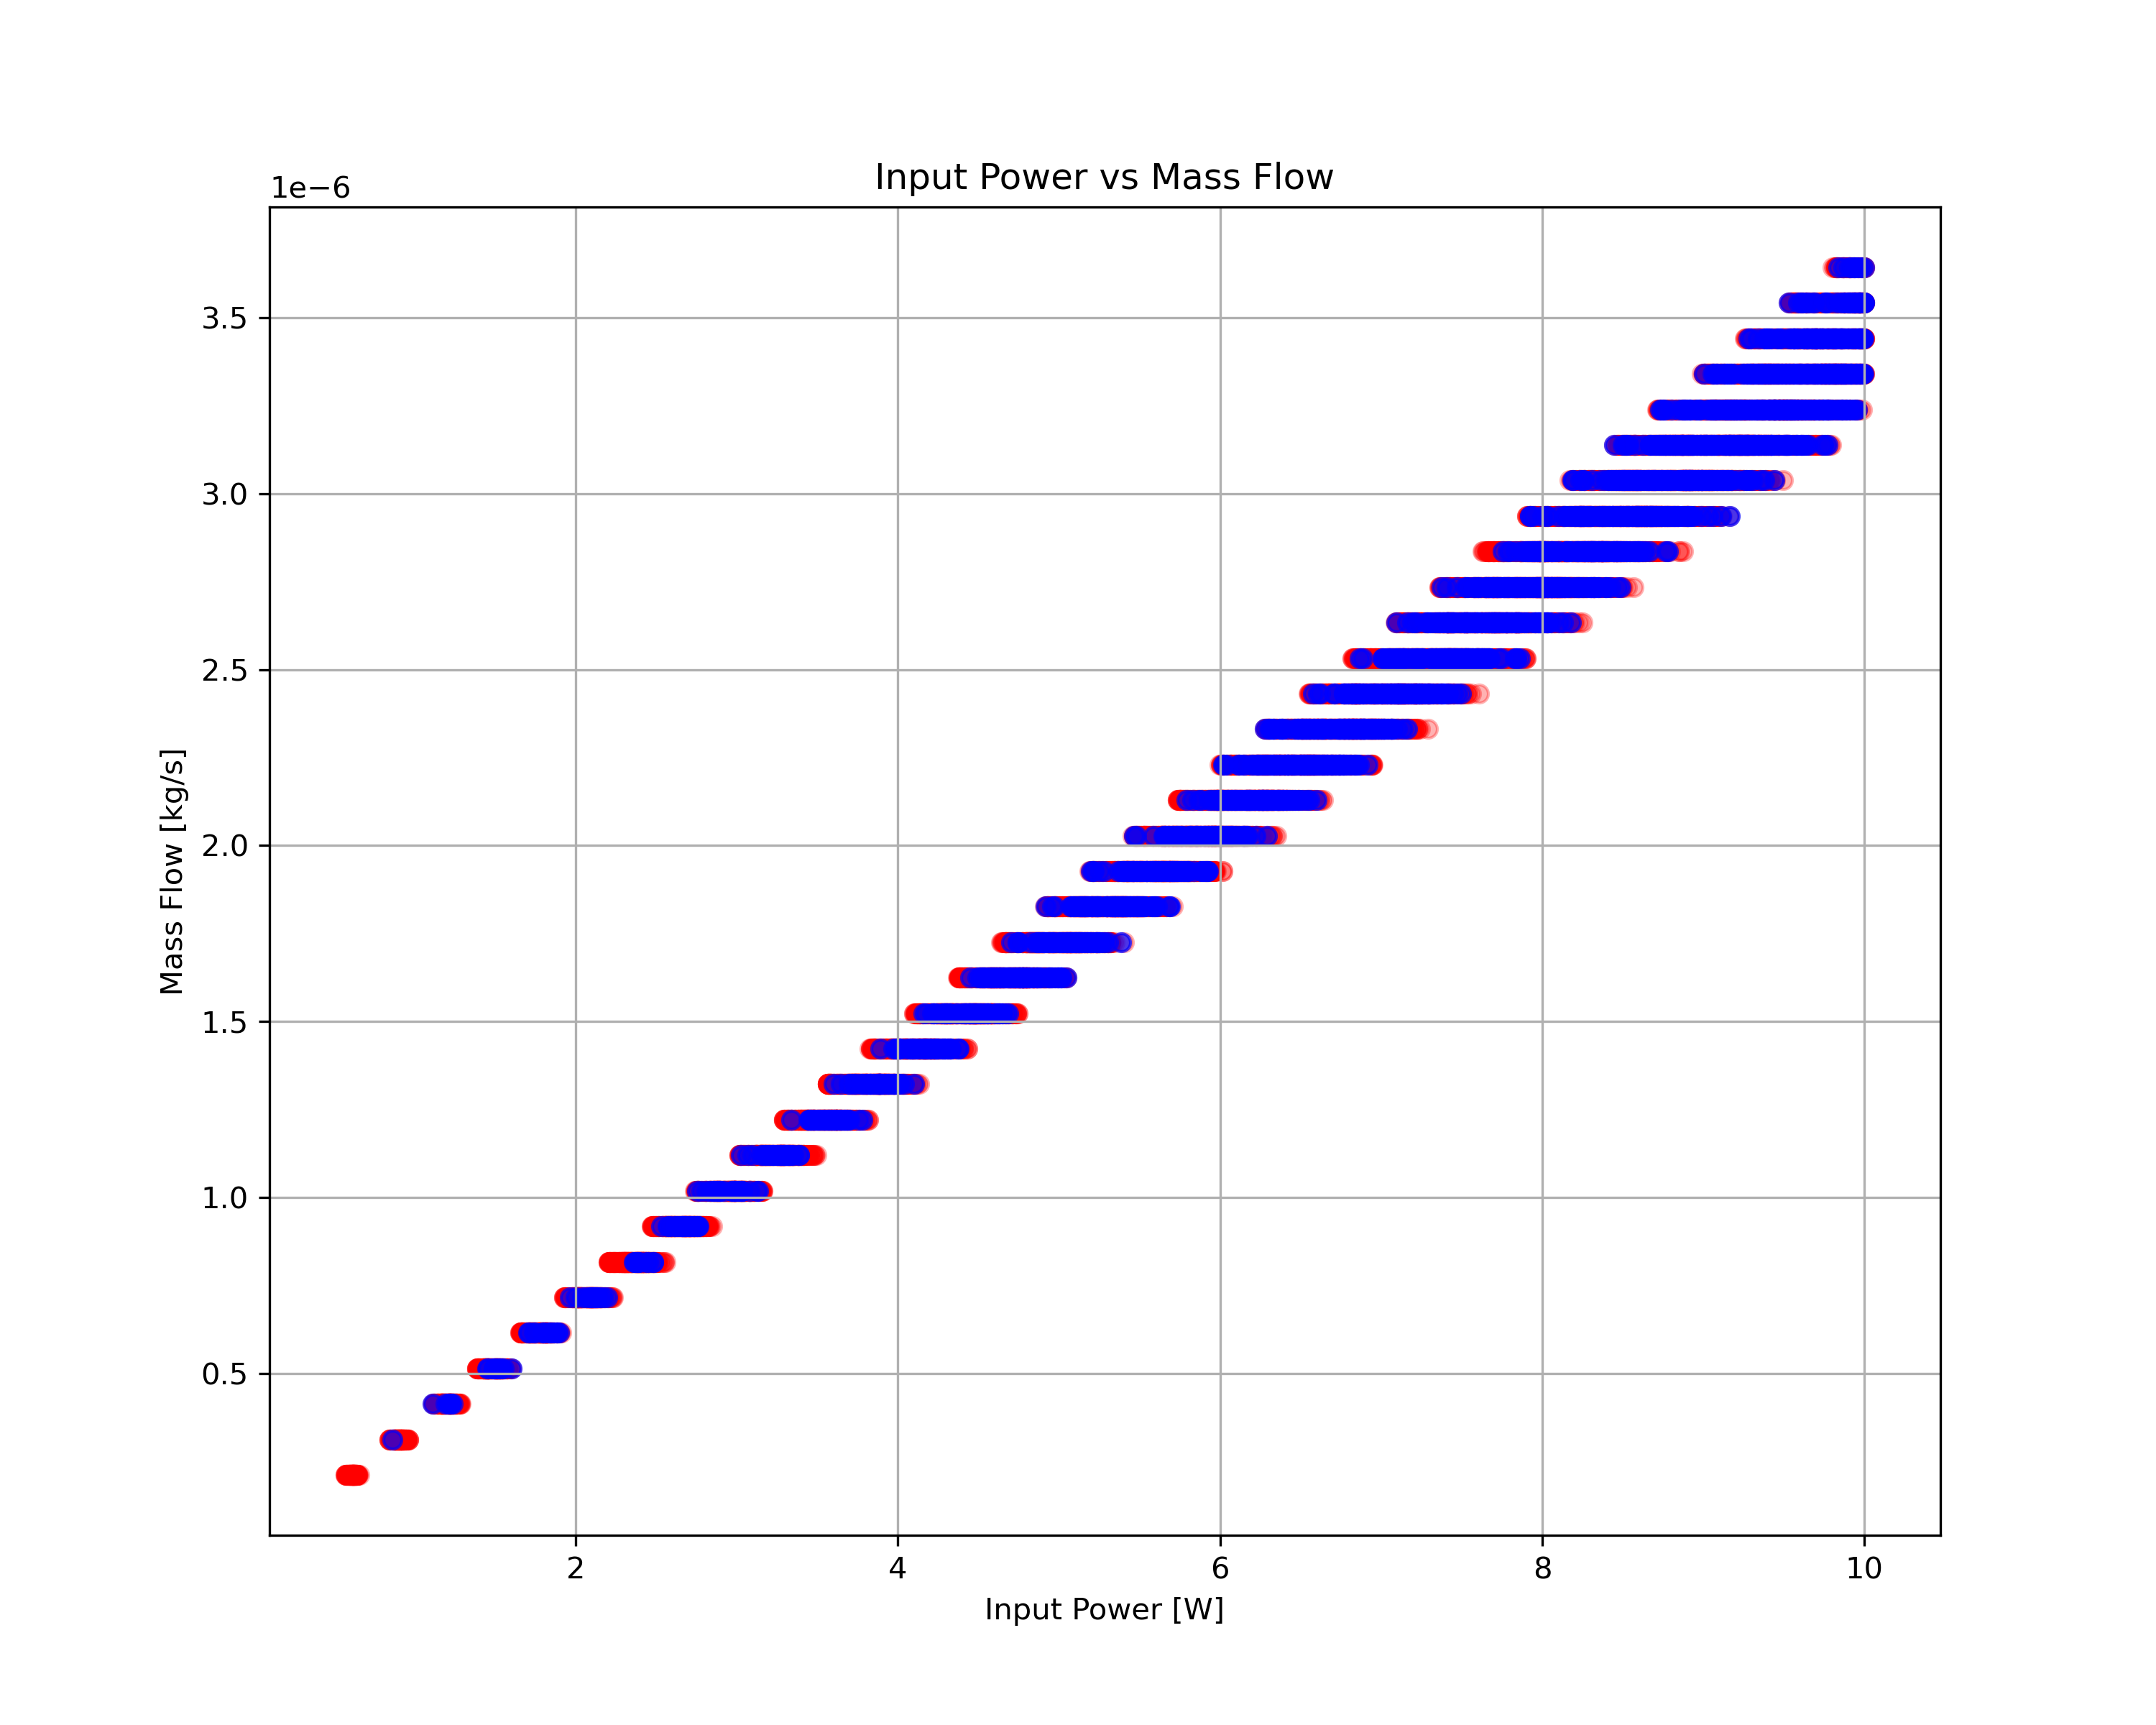
\includegraphics[width=\linewidth]{images/input_power_mass_flow.png}
      \captionof{figure}{Mass Flow vs. Input Power Solutions}
      \label{fig:power_massflow}
  \end{minipage}
  
  \begin{minipage}{\linewidth}
      \centering
      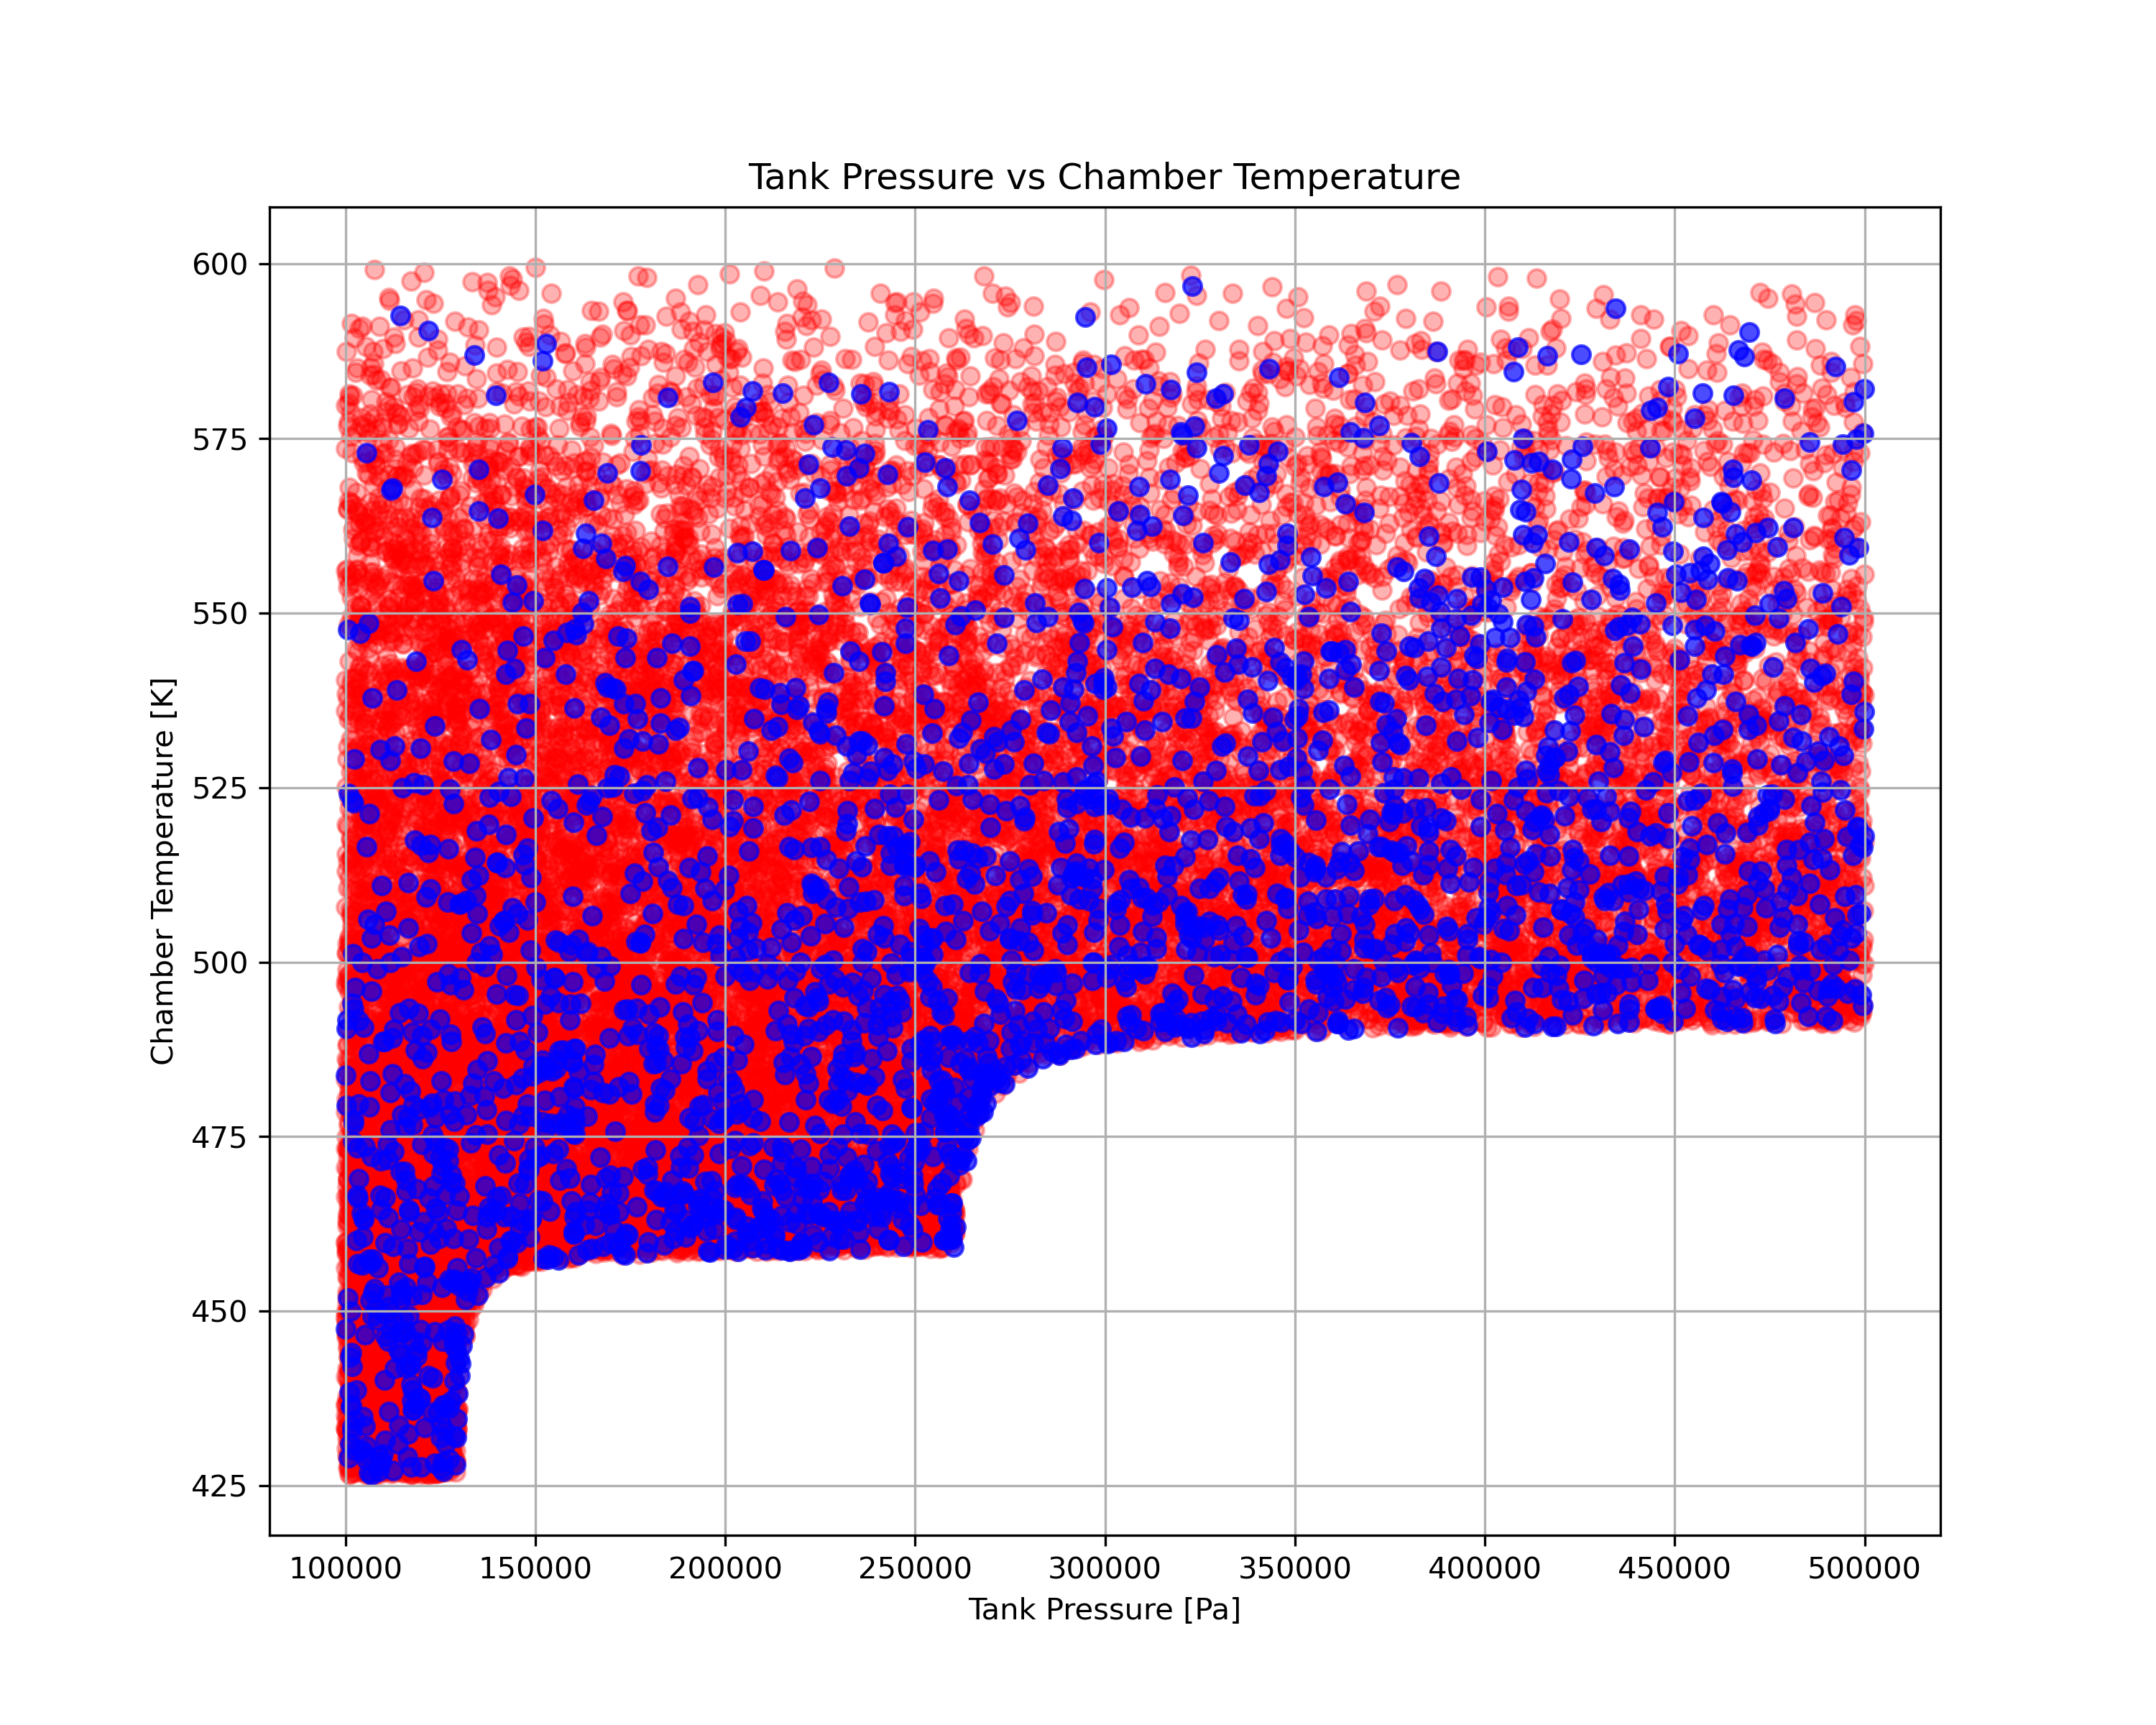
\includegraphics[width=\linewidth]{images/tank_pressure_chamber_temperature_old.png}
      \captionof{figure}{Tank Pressure vs. Chamber Temperature Solutions}
      \label{fig:pressure_temp_old}
  \end{minipage}  
  
  This revealed the actual constraints on physically real solutions for this equation system. These relations were fitted through visual analysis.

    $$ 0.342 \cdot P_{heat} - 0.175  \leq \dot{m} \leq 0.3947 \cdot P_{heat} -0.2 $$ 
  
  $$
  \hspace{-50pt}
  \begin{cases}
    T_c \geq425 & \text{if } 1 \ \text{bar} < p_c < 1.3 \ \text{bar}\\
    T_c \geq 1.8 \cdot \log{p_c - 130000} + 446 & \text{if }1.3 \ \text{bar} < p_c < 2.6 \ \text{bar} \\
   T_c \geq 2.8 \cdot \log{p_c - 260000} + 475 & \text{if } 2.6 \ \text{bar} < p_c < 5 \ \text{bar}
  \end{cases}    
  $$
    
  These constraints were added to the two equation system solver to constrain the search domain for a given calculation. Then, the existence of mass flow and temperature solutions was added as conditions for the generation of a sample using LHS, raising the successful simulation rate from 2.5 to 56 percent. Additionally, the lower limit of the number of heating chamber elements and channels was lowered from 5 to 1. A new set of one hundred thousand samples was generated. Of these, 56,400 were successfully completed, yielding a new dataset with hopefully a more precise look into the domain of interest.

\begin{minipage}{\linewidth} % Use "t" for top placement
\centering
\captionof{table}{Best Design}
\label{tab:best_design}
\begin{tabular}{|c|c|c|}
\hline
\textbf{Parameter} & \textbf{Value} & \textbf{Unit} \\
\hline
Spec. Impulse Efficiency & 0.9815 & \\
Thrust Efficiency & 0.9573 & \\
Nusselt Number & 0.0247 & \\
Discharge Coefficient & 0.9754 & \\
Chamber Reynolds \# & 10.6406 & \\
Mass Flow Error & -0.8166 & mg/s \\
Number of Elements & 1.0 & \\
Number of Channels & 1.0 & \\
Chamber Length & 0.64 & mm \\
Chamber Width & 0.212 & mm \\
Thrust per Power & 0.3985 & mN/W \\
Mass Flow & 3.10 & mg/s \\
Chamber Temperature & 481.5 & K \\
Combined Eval. Par. & 0.6486 & \\
Input Power & 8.8716 & W \\
Tank Pressure & 268042.8 & Pa \\
Nozzle Exit Radius & 99.3 & $\mu$m \\
Throat Radius & 43.6 & $\mu$m \\
Chamber Depth & 391 & $\mu$m \\
Chip Temperature & 498.1 & K \\
Nozzle Length & 8.28 & mm \\
\hline
\end{tabular}
\end{minipage}

A cursory look at the difference a more complete exploration of the design space made is by analysing the delta from the re-design as shown in Table \ref{tab:deltas}.


\begin{table*}[t] % Use "t" for top placement
\centering
\caption{Comparison between Initial Best Design and New Best Design}
\label{tab:deltas}
\begin{tabular}{|c|c|c|c|c|c|}
\hline
\textbf{Parameter} & \textbf{Initial Value} & \textbf{New Value} & \textbf{Absolute $\Delta$} & \textbf{Relative $\Delta$ (\%)} & \textbf{Unit} \\
\hline
Spec. Impulse Efficiency & 0.990 & 0.9862 & 0.0038 & -0.38 & \\
Thrust Efficiency & 0.935 & 0.9211 & 0.0139 & -1.49 & \\
Nusselt Number & $9.9 \times 10^{-4}$ & $0.0002$ & $7.7 \times 10^{-4}$ & -77.78 & \\
Discharge Coefficient & 0.944 & 0.9340 & 0.0100 & -1.06 & \\
Chamber Reynolds \# & 3.03 & 10.6406 & 7.6106 & 250.63 & \\
Mass Flow Error & -1.73 & -0.8166 & 0.9134 & -52.82 & mg/s \\
Chamber Length & 3.2 & 0.64 & 2.56 & -80.00 & mm \\
Chamber Width & 1.06 & 0.212 & 0.848 & -79.81 & mm \\
Thrust per Power & 0.417 & 0.3985 & 0.0185 & -4.43 & mN/W \\
Mass Flow & 3.14 & 3.10 & -0.04 & -1.27 & mg/s \\
Chamber Temperature & 510.5 & 481.5 & 29.0 & -5.68 & K \\
Combined Eval. Par. & 0.654 & 0.6486 & 0.0054 & -0.82 & \\
Input Power & 9.21 & 8.8716 & 0.3384 & -3.67 & W \\
Tank Pressure & 3.275 & 2.68 & 0.595 & -18.17 & Pa \\
Nozzle Exit Radius & 97.6 & 99.3 & 1.7 & 1.74 & $\mu$m \\
Throat Radius & 31.4 & 43.6 & 12.2 & 38.85 & $\mu$m \\
Number of Elements & 5.00 & 1.0 & 4.00 & -80.00 & \\
Number of Channels & 5.00 & 1.0 & 4.00 & -80.00 & \\
Chamber Depth & 215.8 & 391 & 175.2 & 81.10 & $\mu$m \\
Chip Temperature & 537.5 & 498.1 & 39.4 & -7.35 & K \\
Nozzle Length & 8.13 & 8.28 & 0.15 & 1.84 & mm \\
\hline
\end{tabular}
\end{table*}

\subsection{Sensitivity Analysis}

An attempt at a sensitivity analysis was made by fixing all input parameters to those of the best design and sweeping a given parameter over its design range, but because of the narrow range of possible solutions for the mass flow and heating power equation system, rarely any exact mass flow solutions with the required error tolerance ($10^{-1}$ mg/s) were found using this procedure. 

Instead, a sensitivity analysis of the weights used for each evaluation parameter was performed. For every parameter, a truncated normal distribution of values around its original value was created - the truncation ensuring that a negative weight will not become positive and vice versa. These normal distributions' density functions were used to create new weight values for each parameter, for every modification, the other weights were readjusted to keep their relative proportions and keep the sum of the absolute weights at 1.0 using the following steps:

Calculate the difference between the new weight value \(w_{\text {new }}\) and the original weight value \(w_{\text {original: }}\)
$$
\Delta \text{ Weight}=\left|w_{\text {new }}\right|-\left|w_{\text {original }}\right|
$$
Determine the total combined absolute weight of all other weights in the dictionary, excluding the weight under adjustment.
$$
\text { Sum of other weights }=\sum_{k \neq \text { key }}\left|w_k\right|
$$

For the weight associated with the key \(w_{\text {key }}\), assign it the new weight value \(w_{\text {new }}\).
For all other weights \(w_k\) (where \(k \neq \mathrm{key}\) ), proportionally adjust their values to preserve their relative proportions within the dictionary while accommodating the change in \(w_{\text {key }}\).

$$
w_k=w_k-\left(\frac{w_k}{\text { Sum of other weights }}\right) \times \Delta \text{ Weight}
$$

The cluster of the top 10 designs for each new combination of weights was found, and plotted to investigate how sensitive the evaluation parameters are to changes in their own weighting, as shown in Figures \ref{fig:mass_sens}, \ref{fig:nusselt_sens} and \ref{fig:reynolds_sens}. These three parameters were the only ones to have any significant best design response to the changing of their weights. All other parameters maintained constant best designs, although the distribution of the top 10 best designs did chang, similarly to the mass flow, Nusselt number and Reynolds number. This implies that there may be more sensitivity to change than simply choosing the best design may lead to.

  \begin{minipage}{\linewidth}
      \centering
      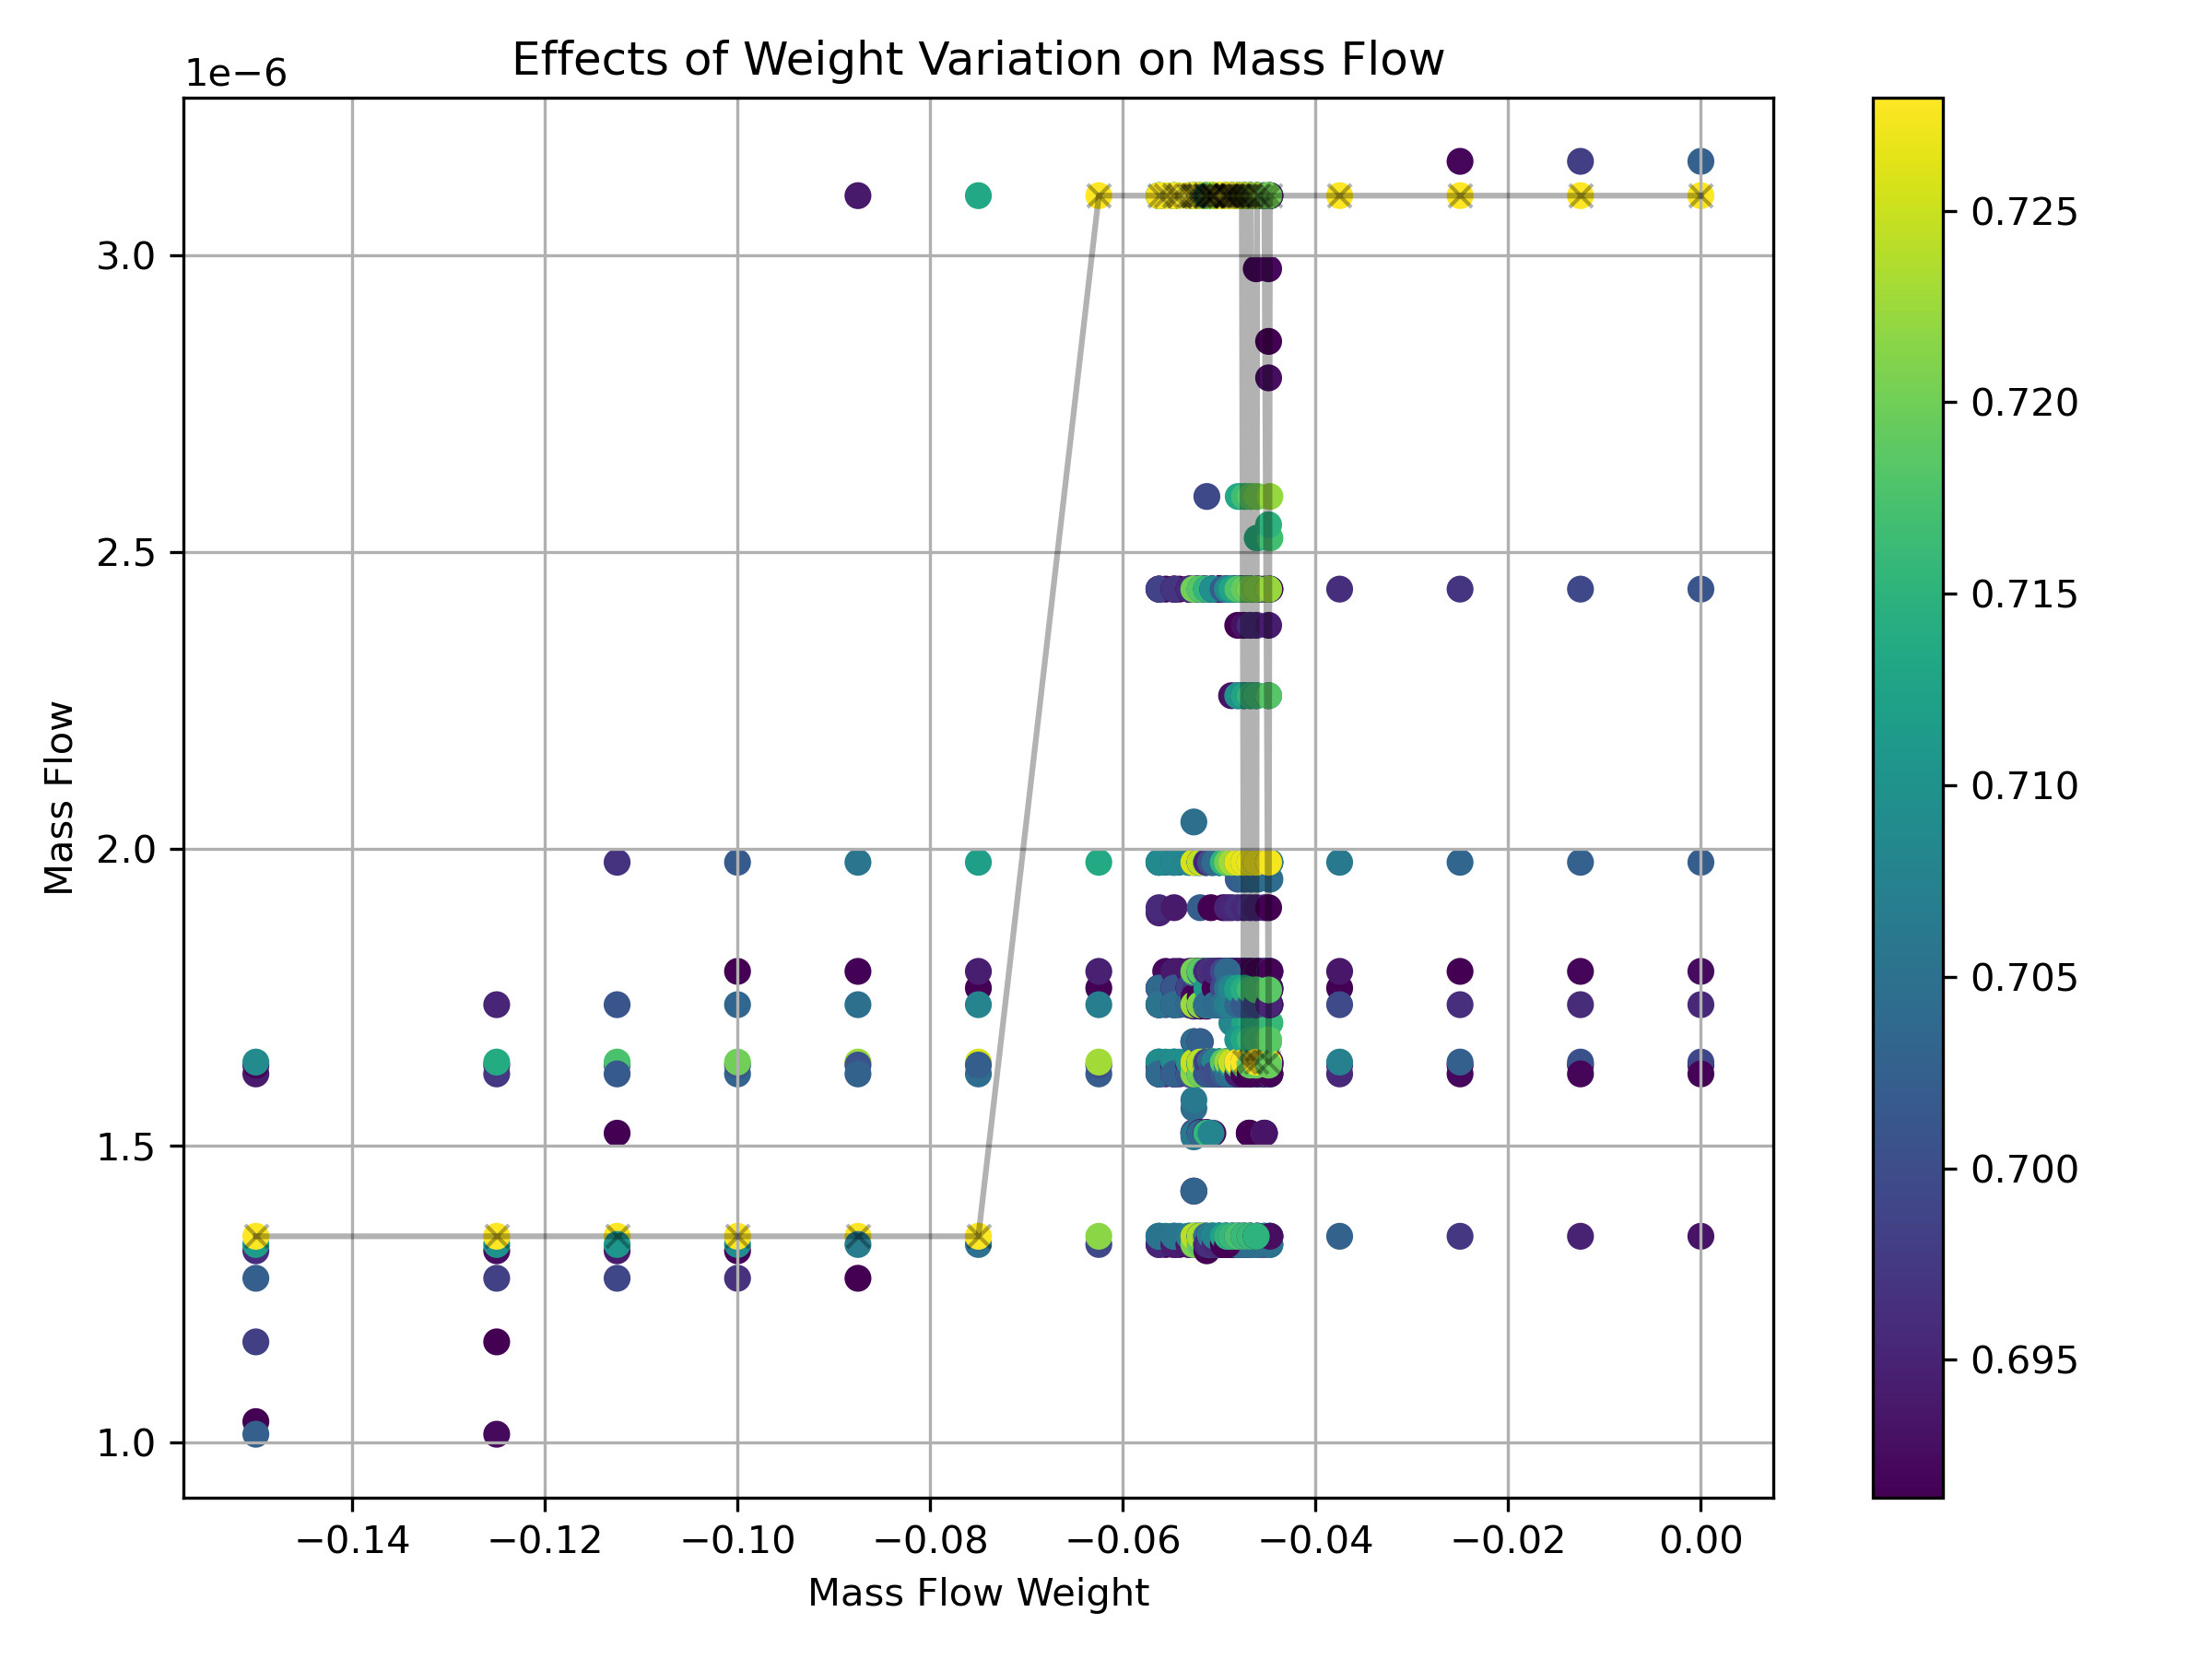
\includegraphics[width=\linewidth]{images/mass_flow_sensitivity.png}
      \captionof{figure}{Mass flow sensitivity analysis}
      \label{fig:mass_sens}
  \end{minipage}  

\begin{minipage}{\linewidth}
  \centering
  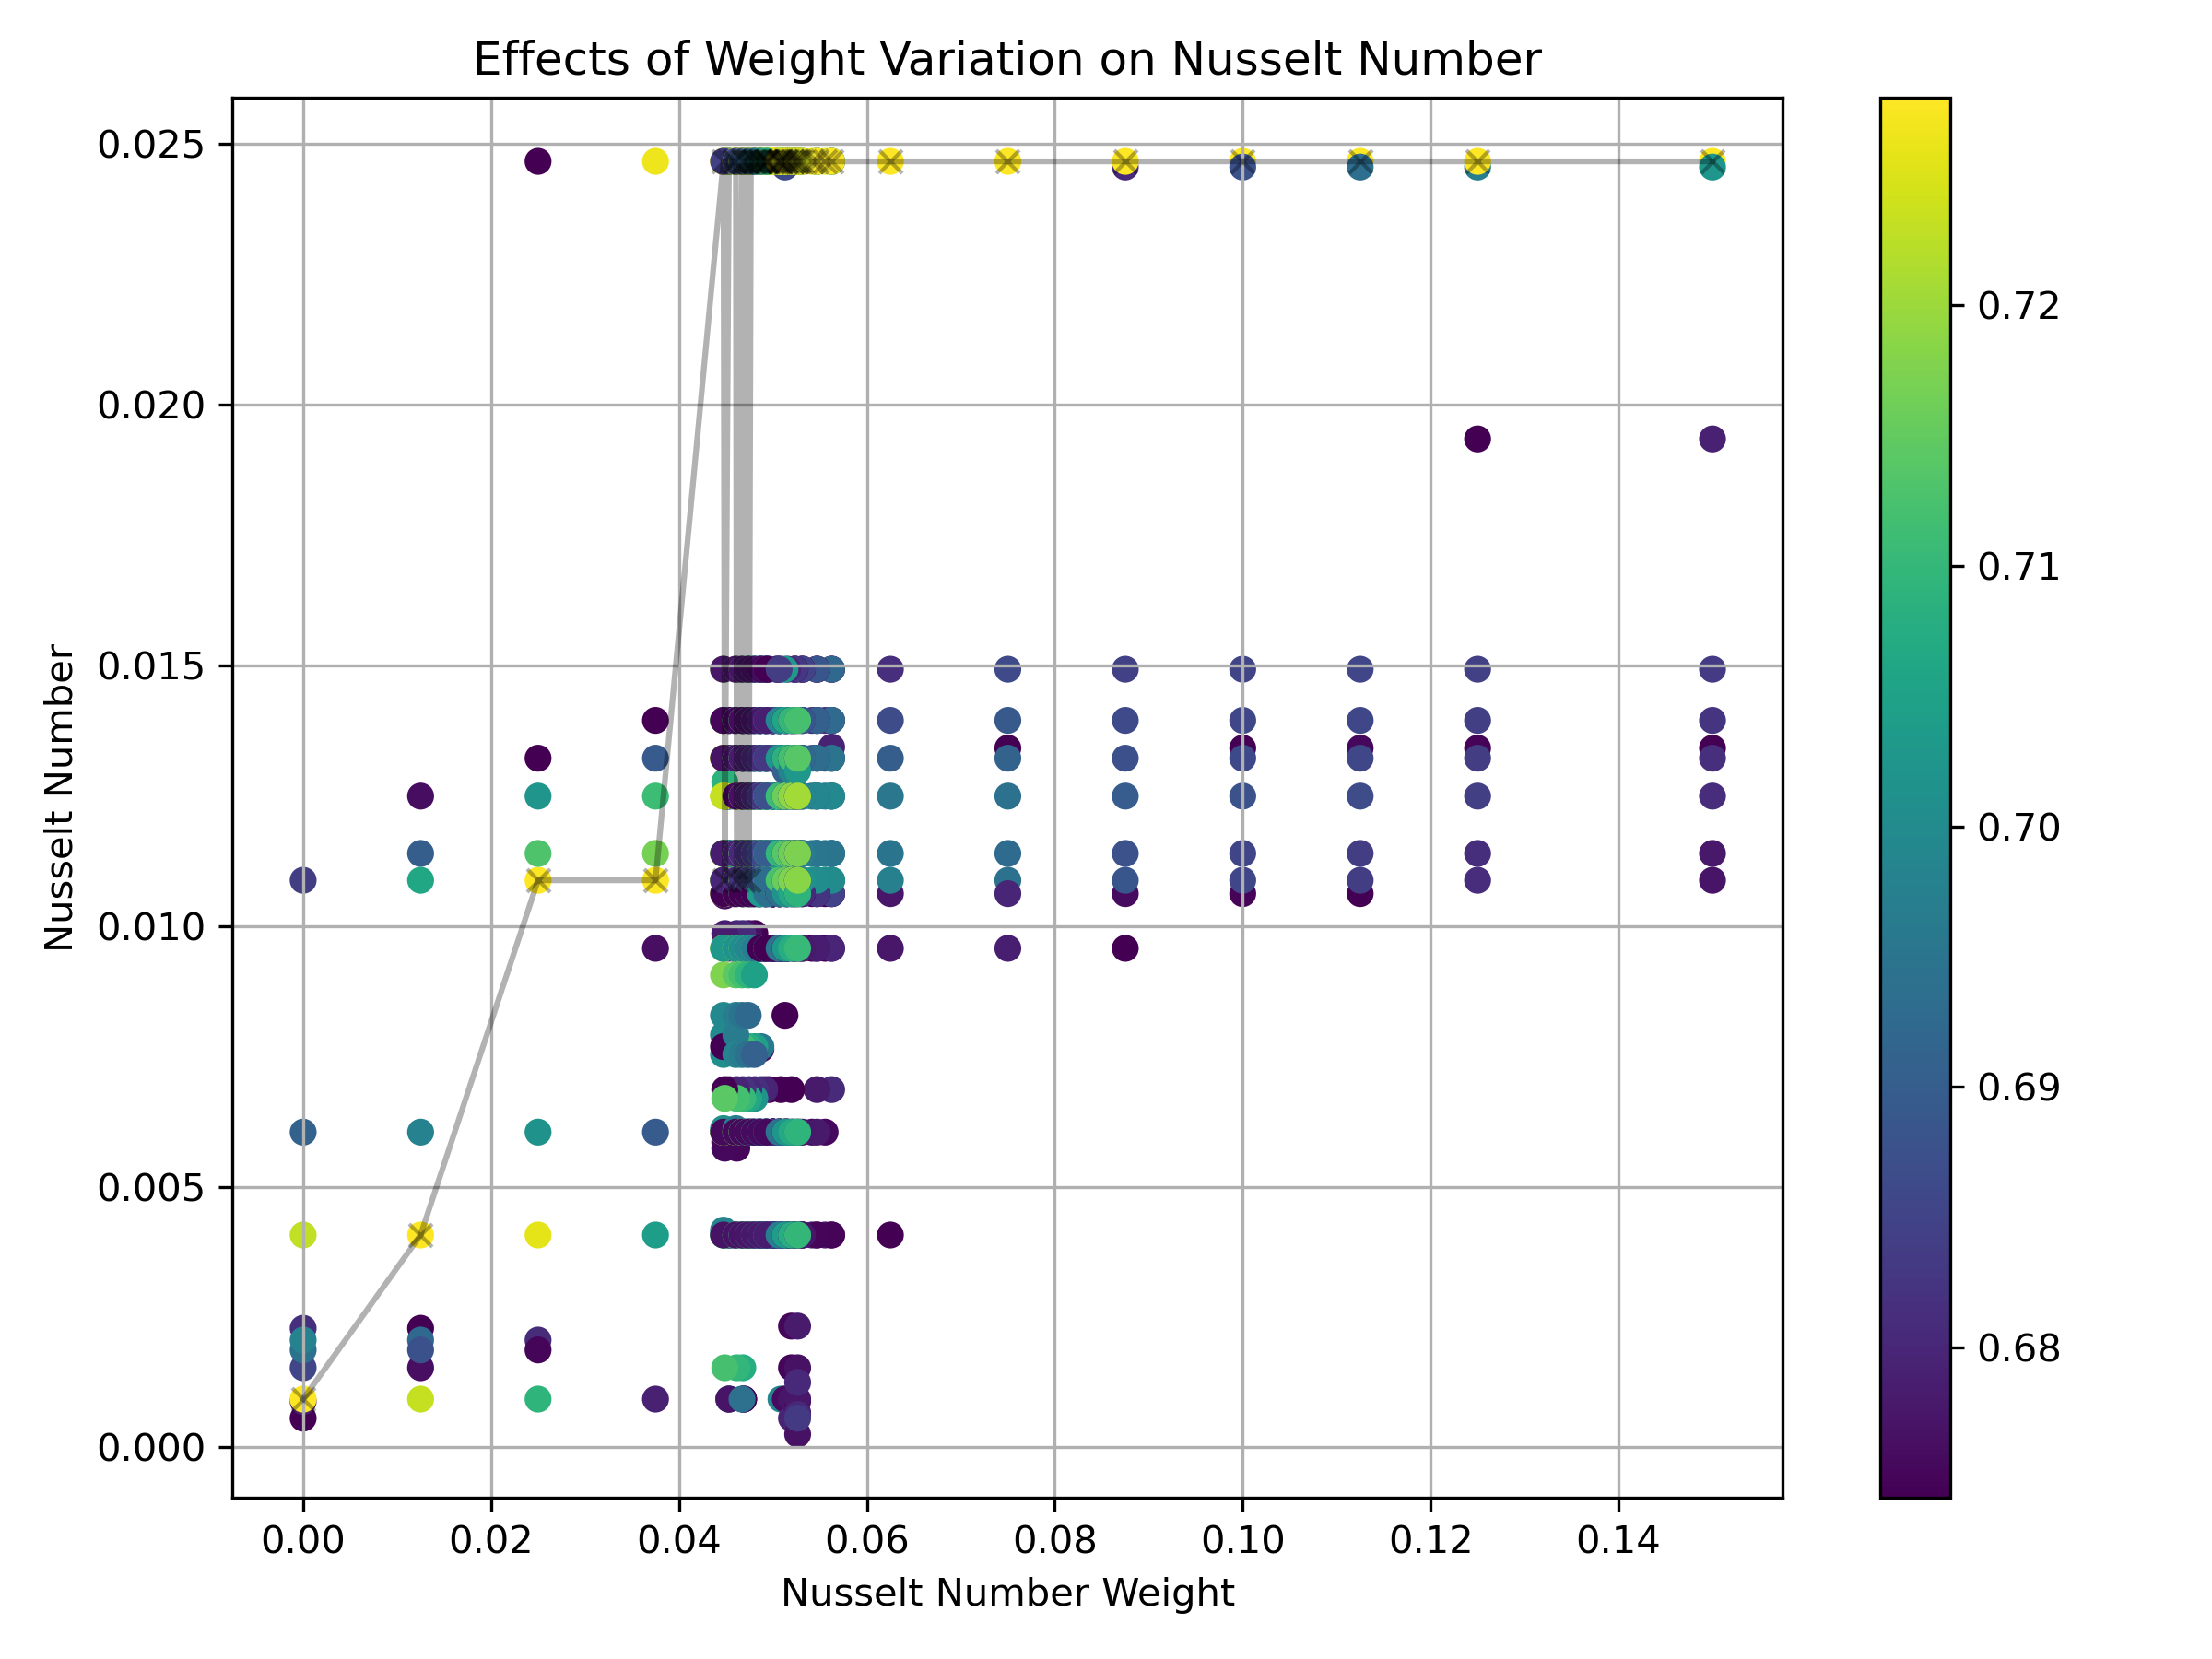
\includegraphics[width=\linewidth]{images/nusselt_number_sensitivity.png}
  \captionof{figure}{Nusselt Number sensitivity analysis}
  \label{fig:nusselt_sens}
\end{minipage} 

  \begin{minipage}{\linewidth}
      \centering
      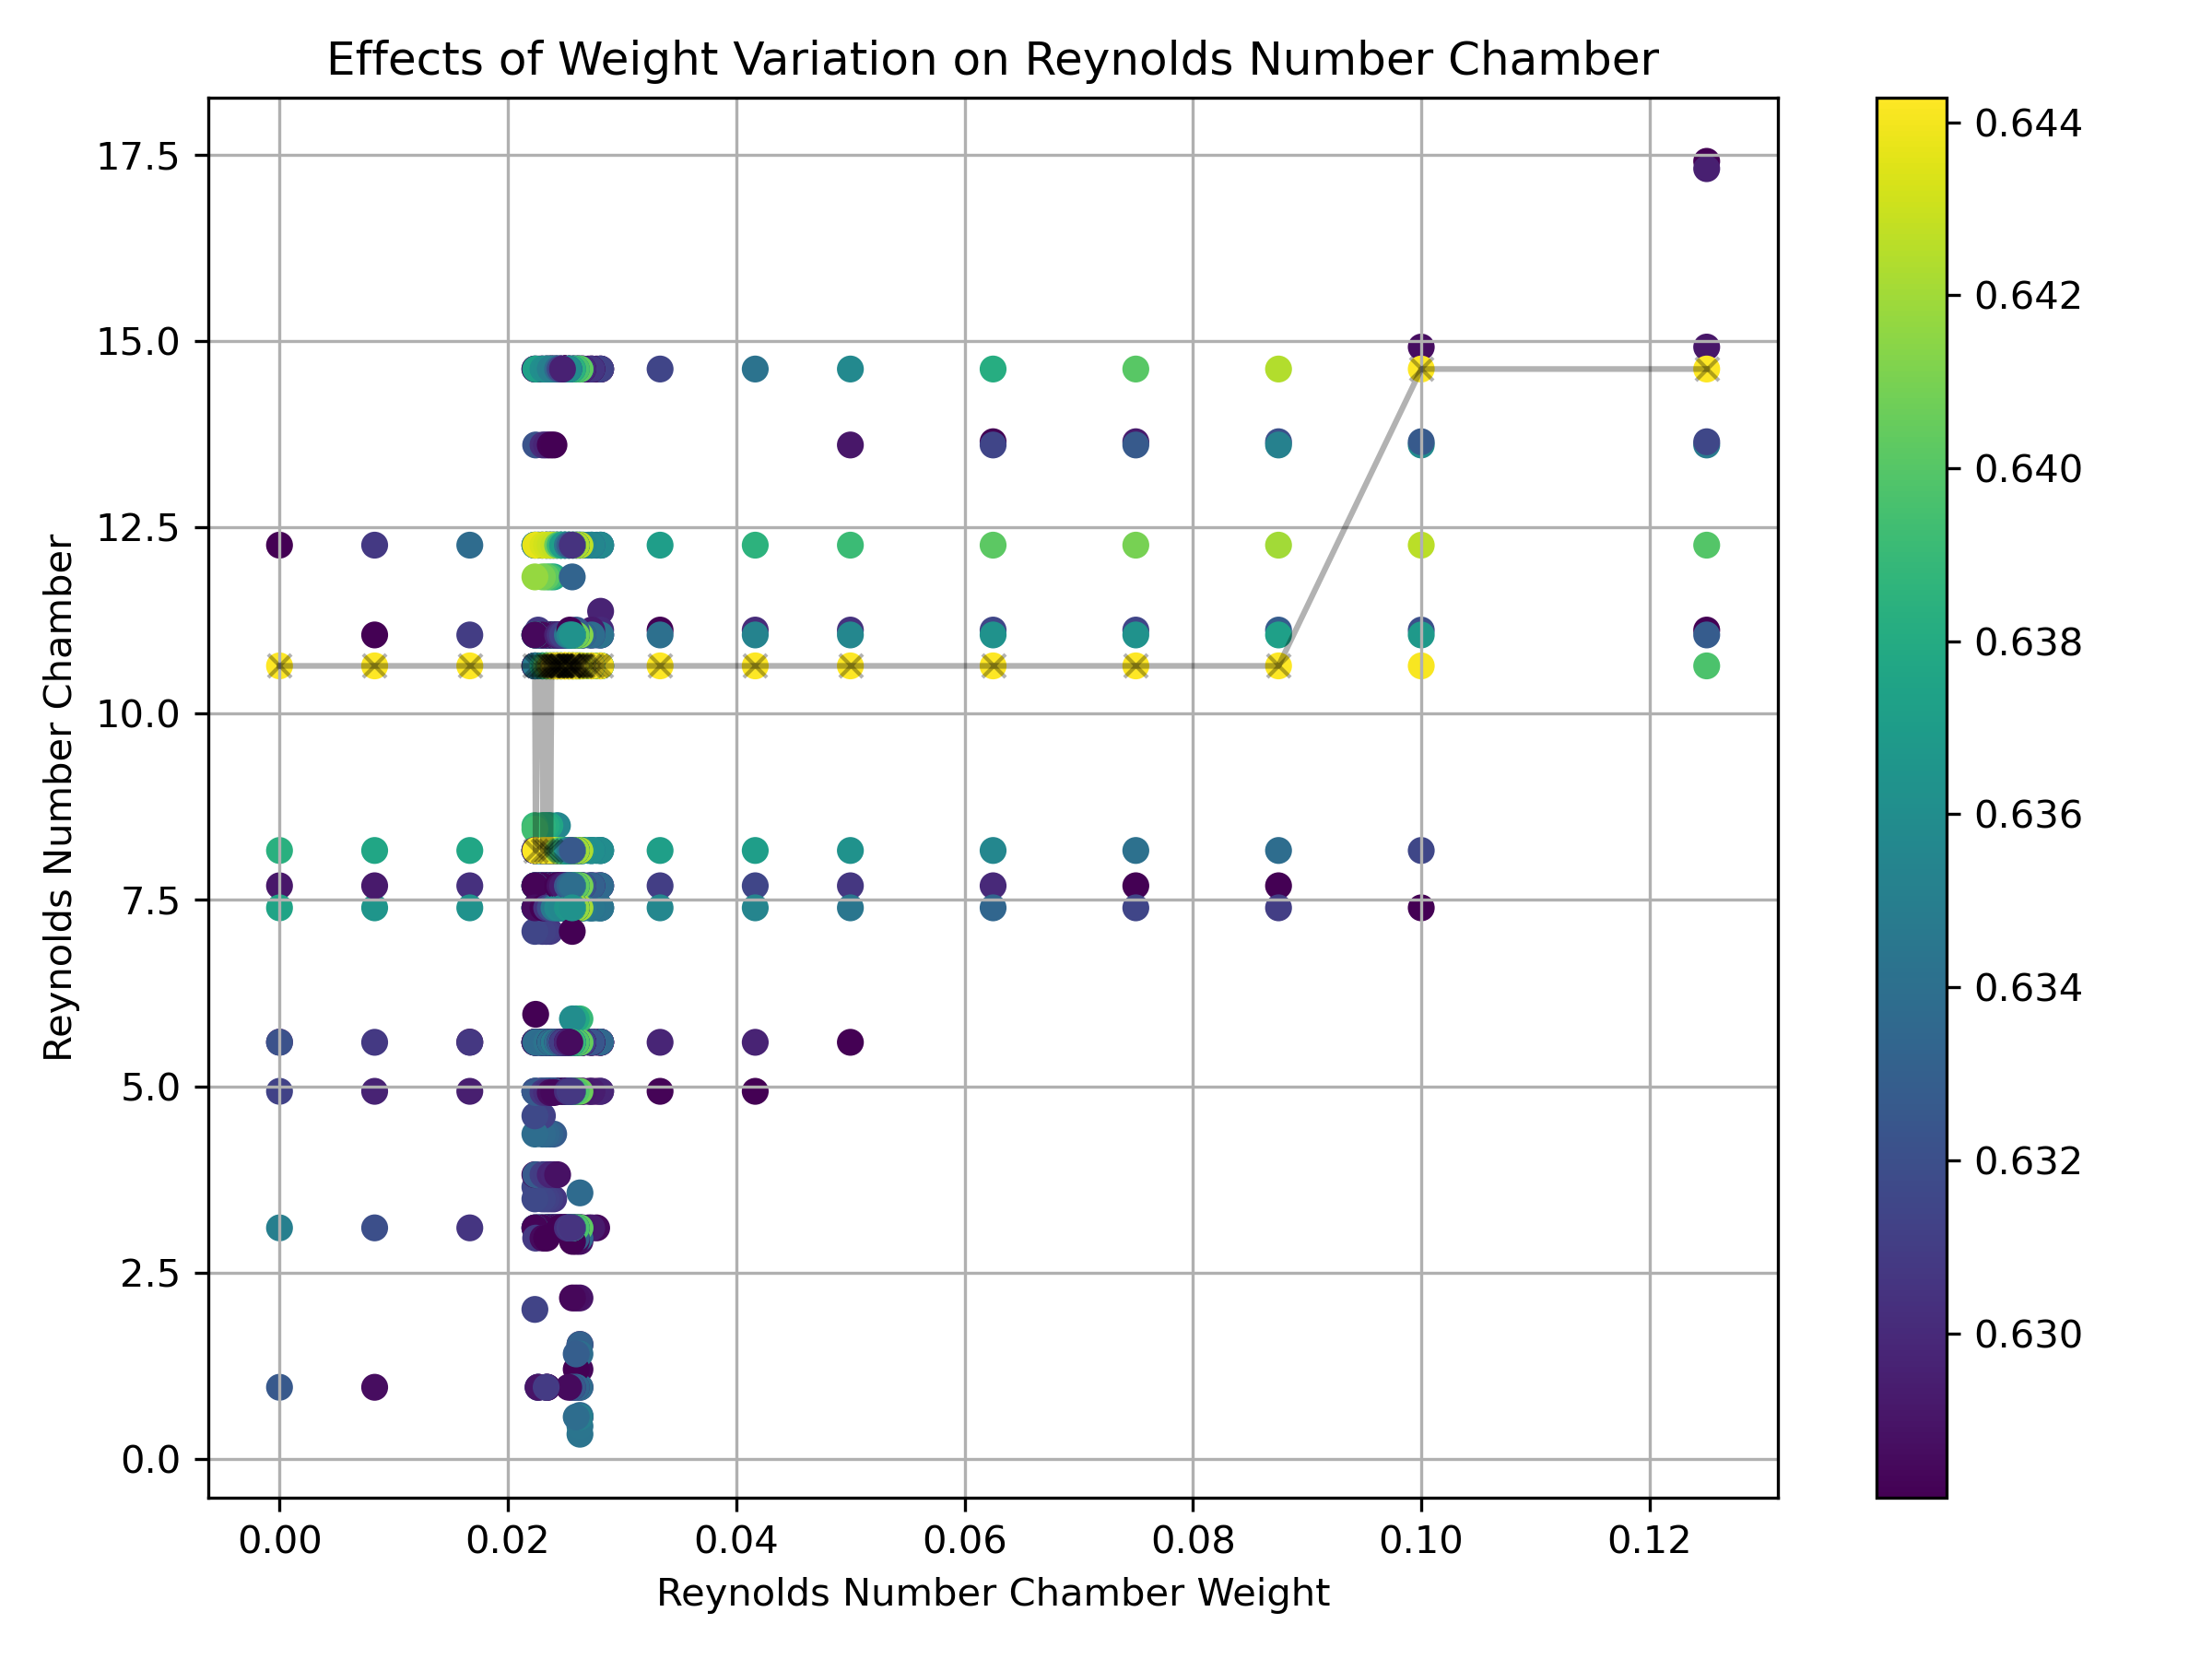
\includegraphics[width=\linewidth]{images/reynolds_number_chamber_sensitivity.png}
      \captionof{figure}{Reynolds number sensitivity analysis}
      \label{fig:reynolds_sens}
  \end{minipage} 


\subsection{Discussion of Parameter Deltas}

In all of the following scatter plots, the top 10 percent in terms of the combined evaluation score as described above are plotted in blue, while the bottom 90 percent are plotted in red. If green points are also present, then they represent the top 1 percent of designs, with yellow representing the top 0.1 percent of designs.

\textbf{Nusselt Number}: The relatively large decrease is negative, suggesting reduced heat transfer efficiency. This may just be the result of a higher heating chamber wall surface area, since the chamber depth also increased by 81\%, even though the number of heating chamber elements and channels was minimized to their lowerst possible value. A higher Nusselt number indicates better convective heat transfer, which is crucial for minimizing the required heating chamber dimensions. However, one of the weak points of the model developed in this paper is precisely the extremely low Nusselt numbers (as well as Reynolds numbers) which are orders of magnitude below their expected range as shown in Figure \ref{fig:power_nusselt}. Although their relative values were used to compare designs, their absolute values are likely not physically meaningful for describing the heat transfer.

\textbf{Discharge Coefficient}: The small increase is positive, implying a more efficient flow through the nozzle due to a smaller boundary layer forming there.

\textbf{Chamber Reynolds \#}: The significant increase is positive, as a lower chamber Reynolds number might lead to smoother flow behavior and improved overall system performance, it also increases the likelihood of boundary layer effects in the heating chamber, specially at these very low Reynolds numbers.

\begin{minipage}{\linewidth}
      \centering
      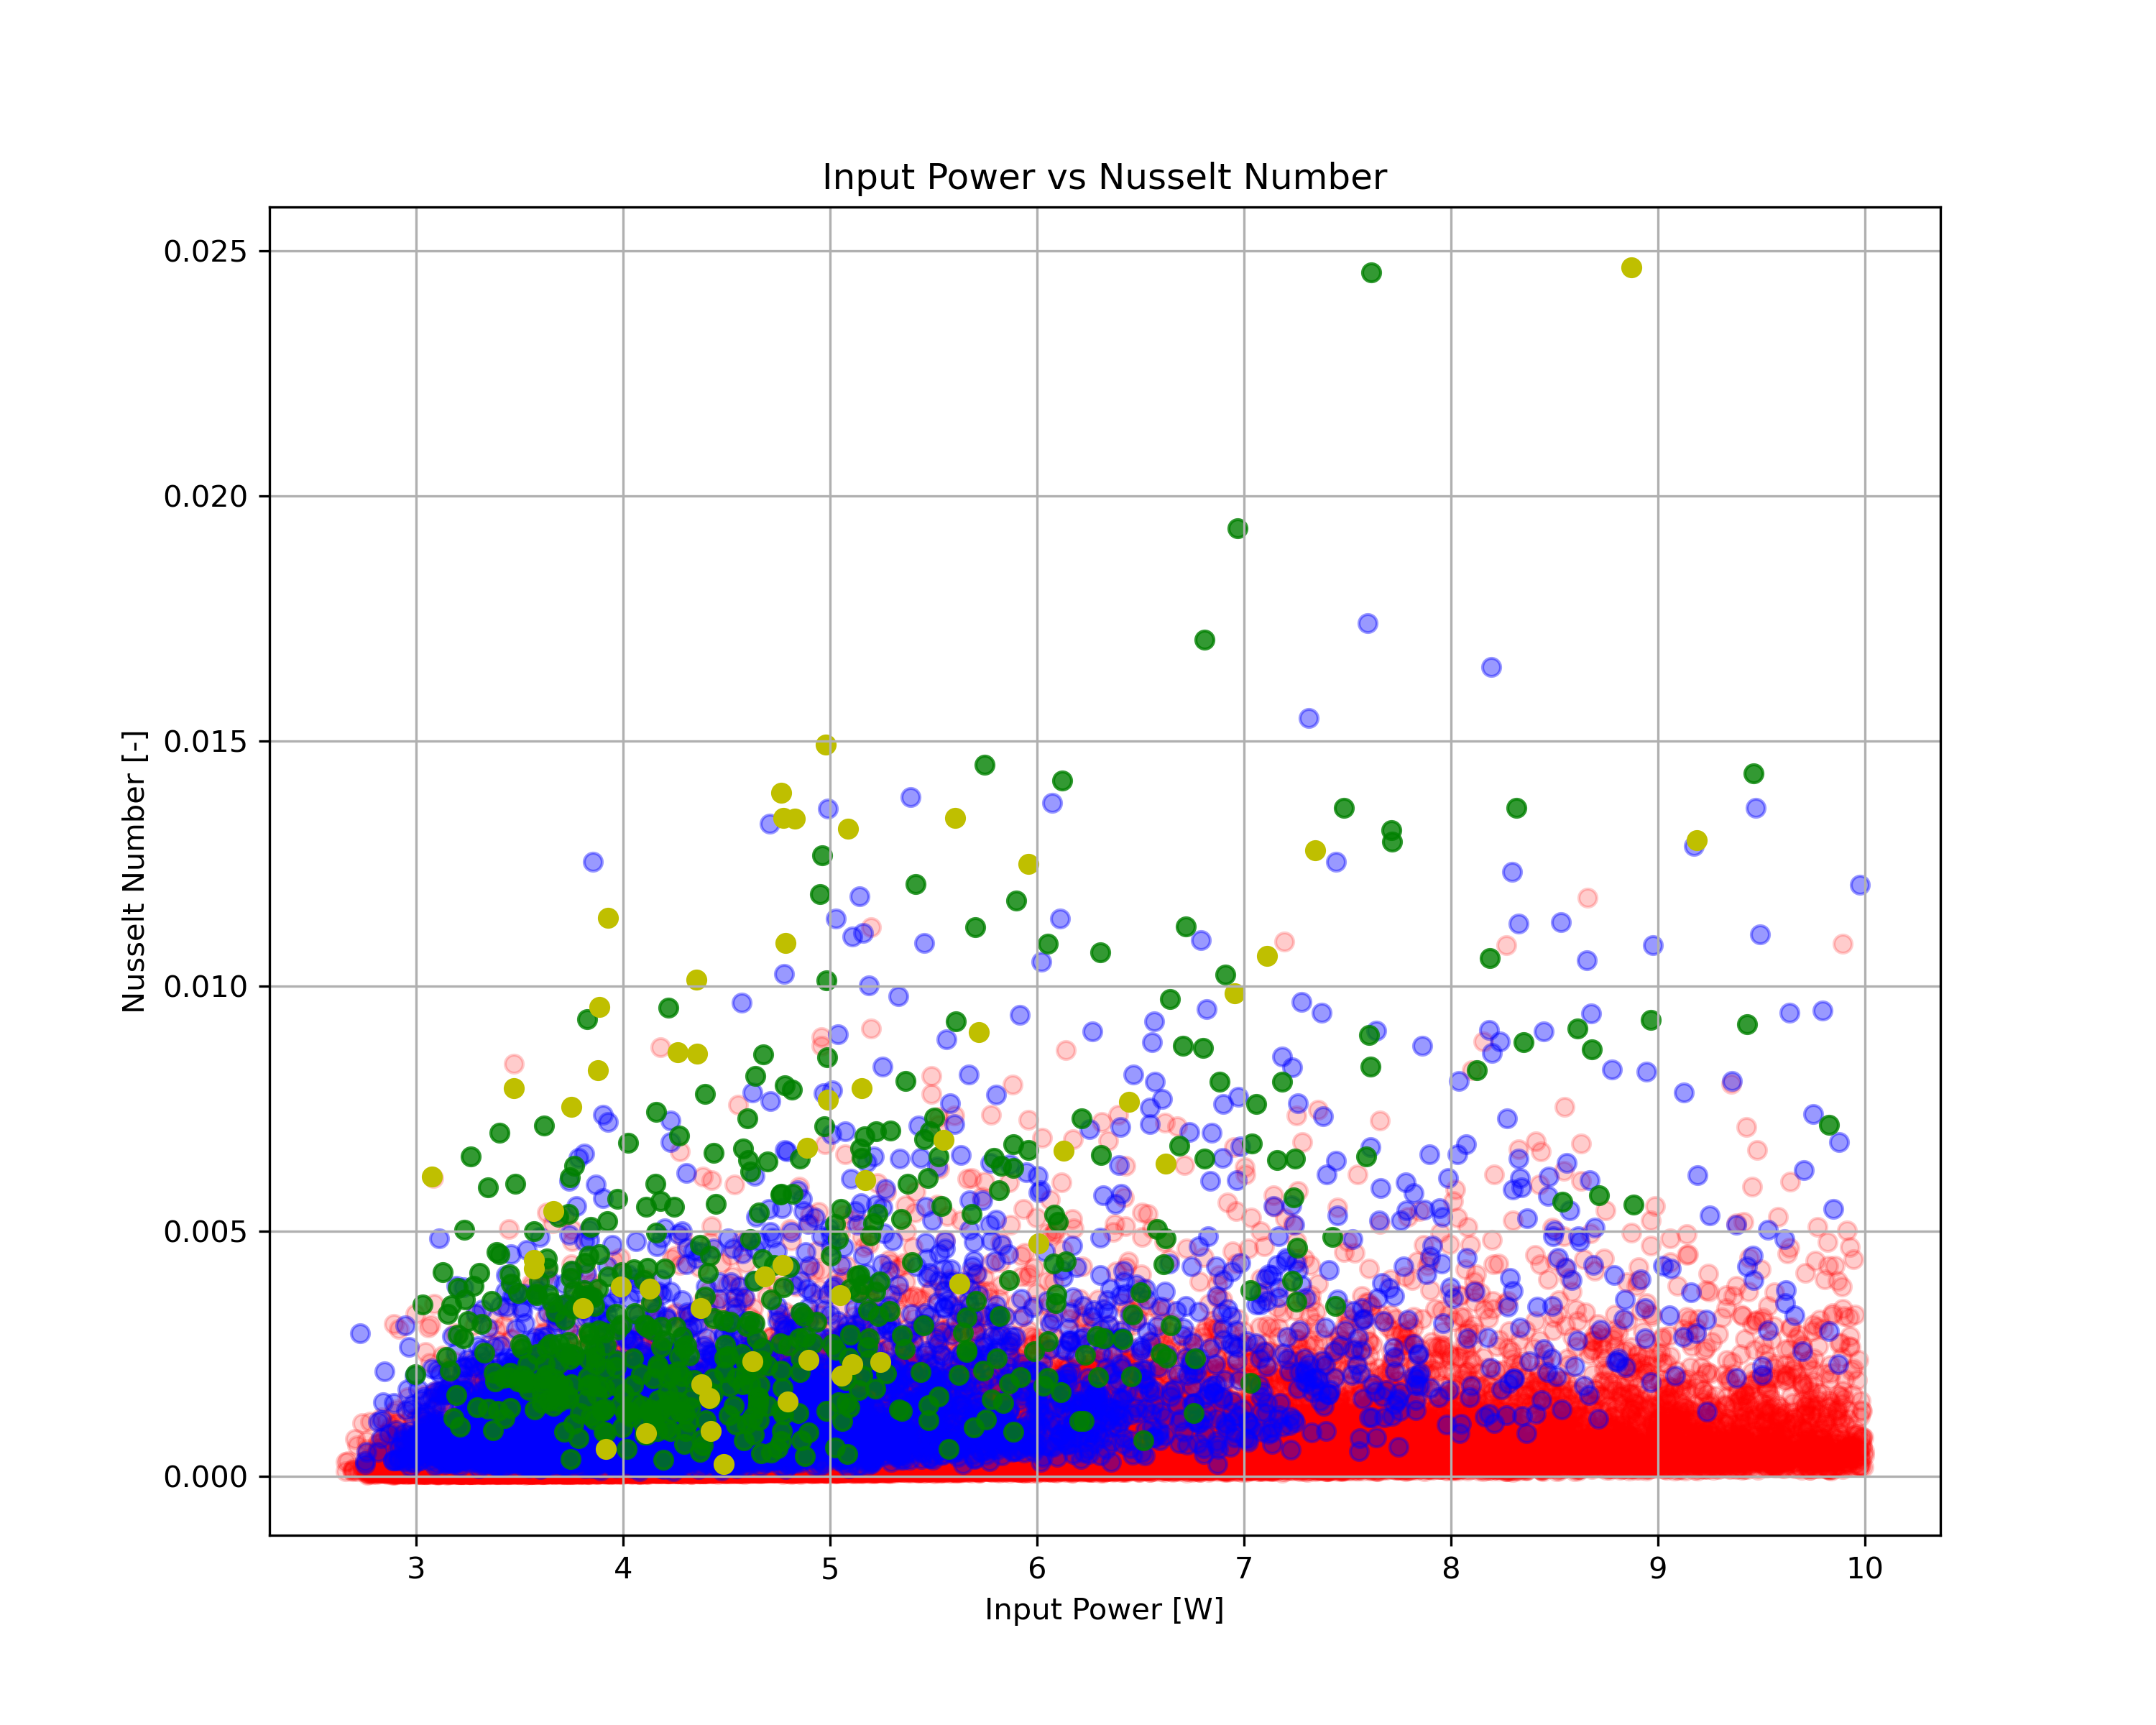
\includegraphics[width=\linewidth]{images/input_power_nusselt_number.png}
      \captionof{figure}{Input Power vs. Nusselt Number}
      \label{fig:power_nusselt}
  \end{minipage}

\textbf{Mass Flow Error}: The significant reduction in calculation error is positive, although this is a product of using a finer calculation mesh due to the reduced grid-search domain the two added mass flow and chamber temperature constraints imposed. All new mass flow errors were at most 1 mg/s, but ideally, one should aim for at most a 0.01 mg/s error in calculation.

\textbf{Chamber Length and Width}: The change in the chamber length and width is due to the alteration of the lower limit of the number of heating elements and channels from 5 to 1 in the recalculation. Since these parameters are to be minimized, it makes sense that they would be near the bottom of their ranges, but the current best version of the design has a strange shape where the heating chamber is much smaller than the nozzle, which is a questionable arrangement in comparison with previous designs. The element not considered in this simulation which would likely counteract the minimization of heating chamber surface area is the upper limit of the heat flux that the resistances used and the walls of the heating chamber can achieve. Past a certain surface area, the heat flux will be too high and potentially damage the heating chamber. 

\textbf{Thrust per Power}: The decrease is negative, as more power will be required for the same thrust, although it is still in the expected range. As can be seen in Figure \ref{fig:power_thrust_per}, there were many top 0.01\% designs with thrust per power ratings as high as 0.45 mN/W, but they likely did not win due to worse performance in discharge coefficient or other more heavily weighted parameters.

\begin{minipage}{\linewidth}
      \centering
      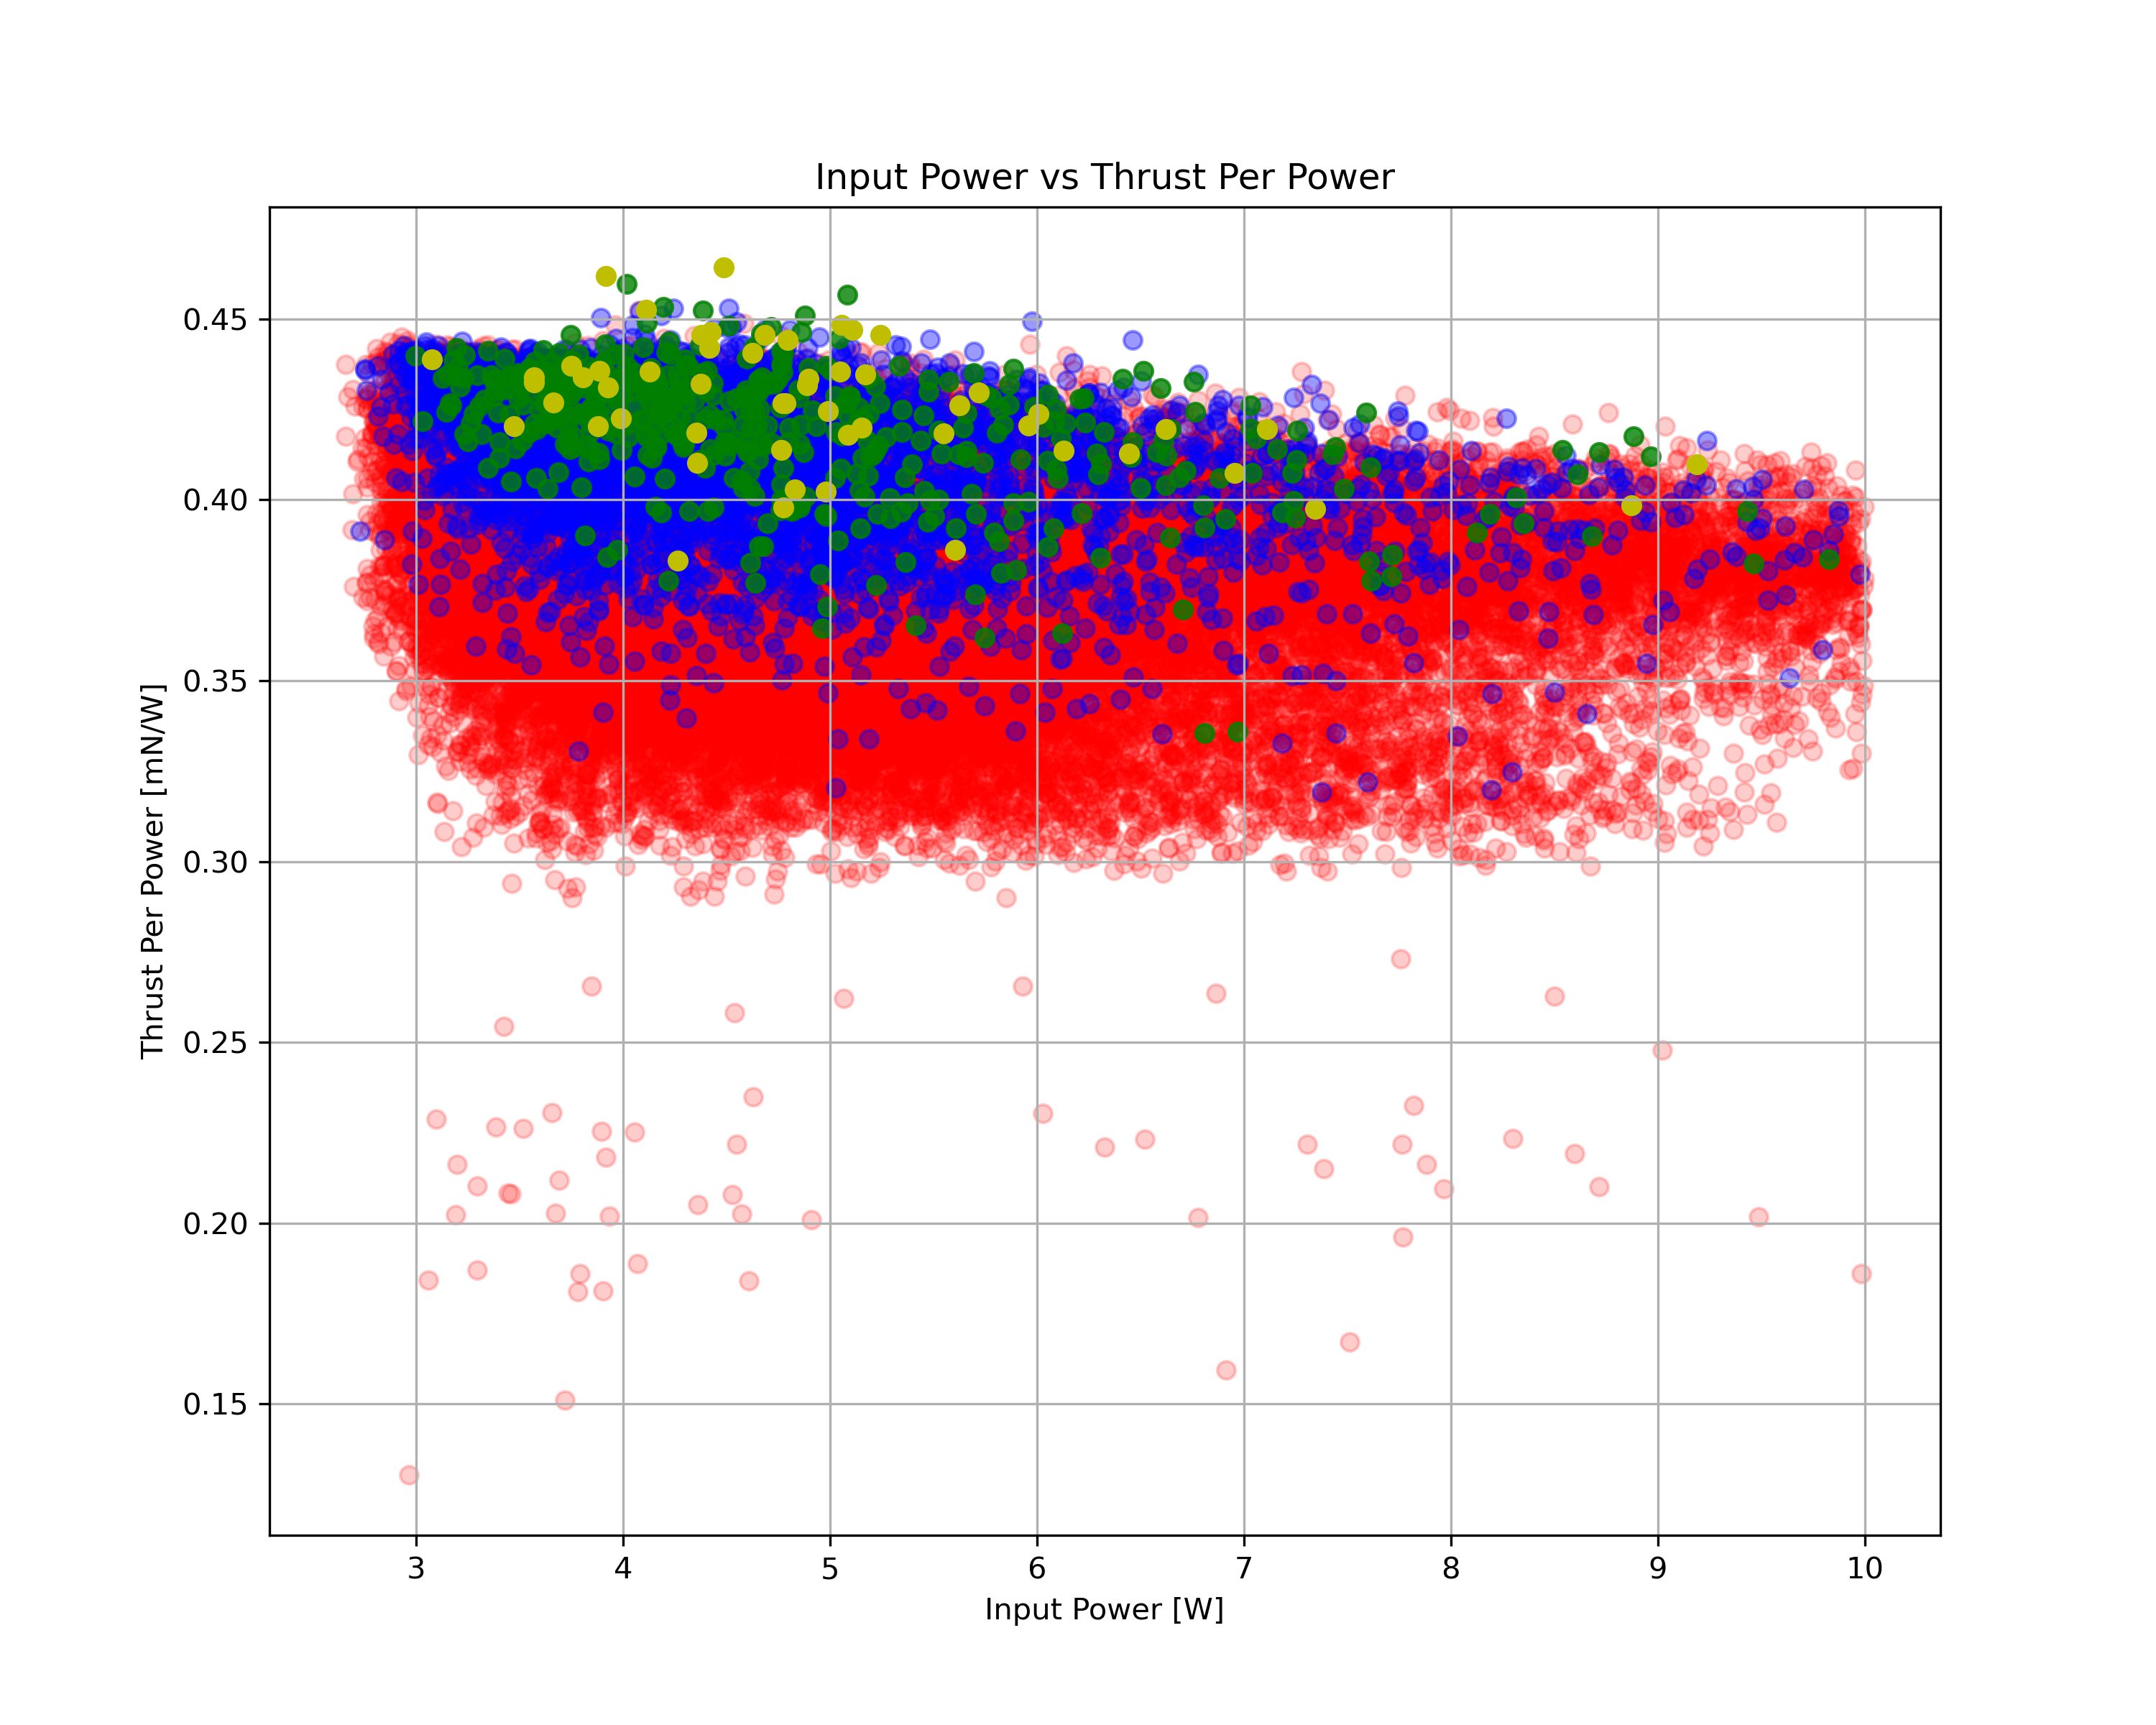
\includegraphics[width=\linewidth]{images/input_power_thrust_per_power.png}
      \captionof{figure}{Input Power vs. Thrust per Power}
      \label{fig:power_thrust_per}
  \end{minipage}

\textbf{Mass Flow}: The significant decrease is positive, indicating reduced consumption of propellant and longer mission durations or reduced propellant mass required.

\textbf{Chamber Temperature}: The decrease is positive, as is that of the Chip (Wall) temperature, as lower temperatures are generally better for spacecraft systems due to lower thermal management complexity, reduced thermal leakage probabilities, and increased component reliability and longevity. Figure \ref{fig:pressure_chamber_temp} shows that the highest performing designs cluster around low temperatures and heating powers, but relatively high pressures. This is likely due to the lower limit of temperature-pressure combinations being that the vapor must remaing gaseous at the exit by not cooling down too much. Perhaps by lowering the temperature of the water in the storage tank, even lower heating chamber temperatures might be achieved, since the high performing cluster is bordering around the limit of physical solutions to the respective equation system.

\textbf{Input Power}: The small relative decrease is positive, since lower heating power requirements contribute to longer operational capabilities and energy savings. Figure \ref{fig:power_chamber_temp} shows that lower heating powers perform better (combined with high pressures). Remembering the quasi-linear relationship between mass flow and input power, this indicates that low mass flows perform better, which intuitively makes sense in the heating chamber: a slowly flowing, highly pressure liquid will need less power to heat it in a smaller volume.

\begin{minipage}{\linewidth}
  \centering
  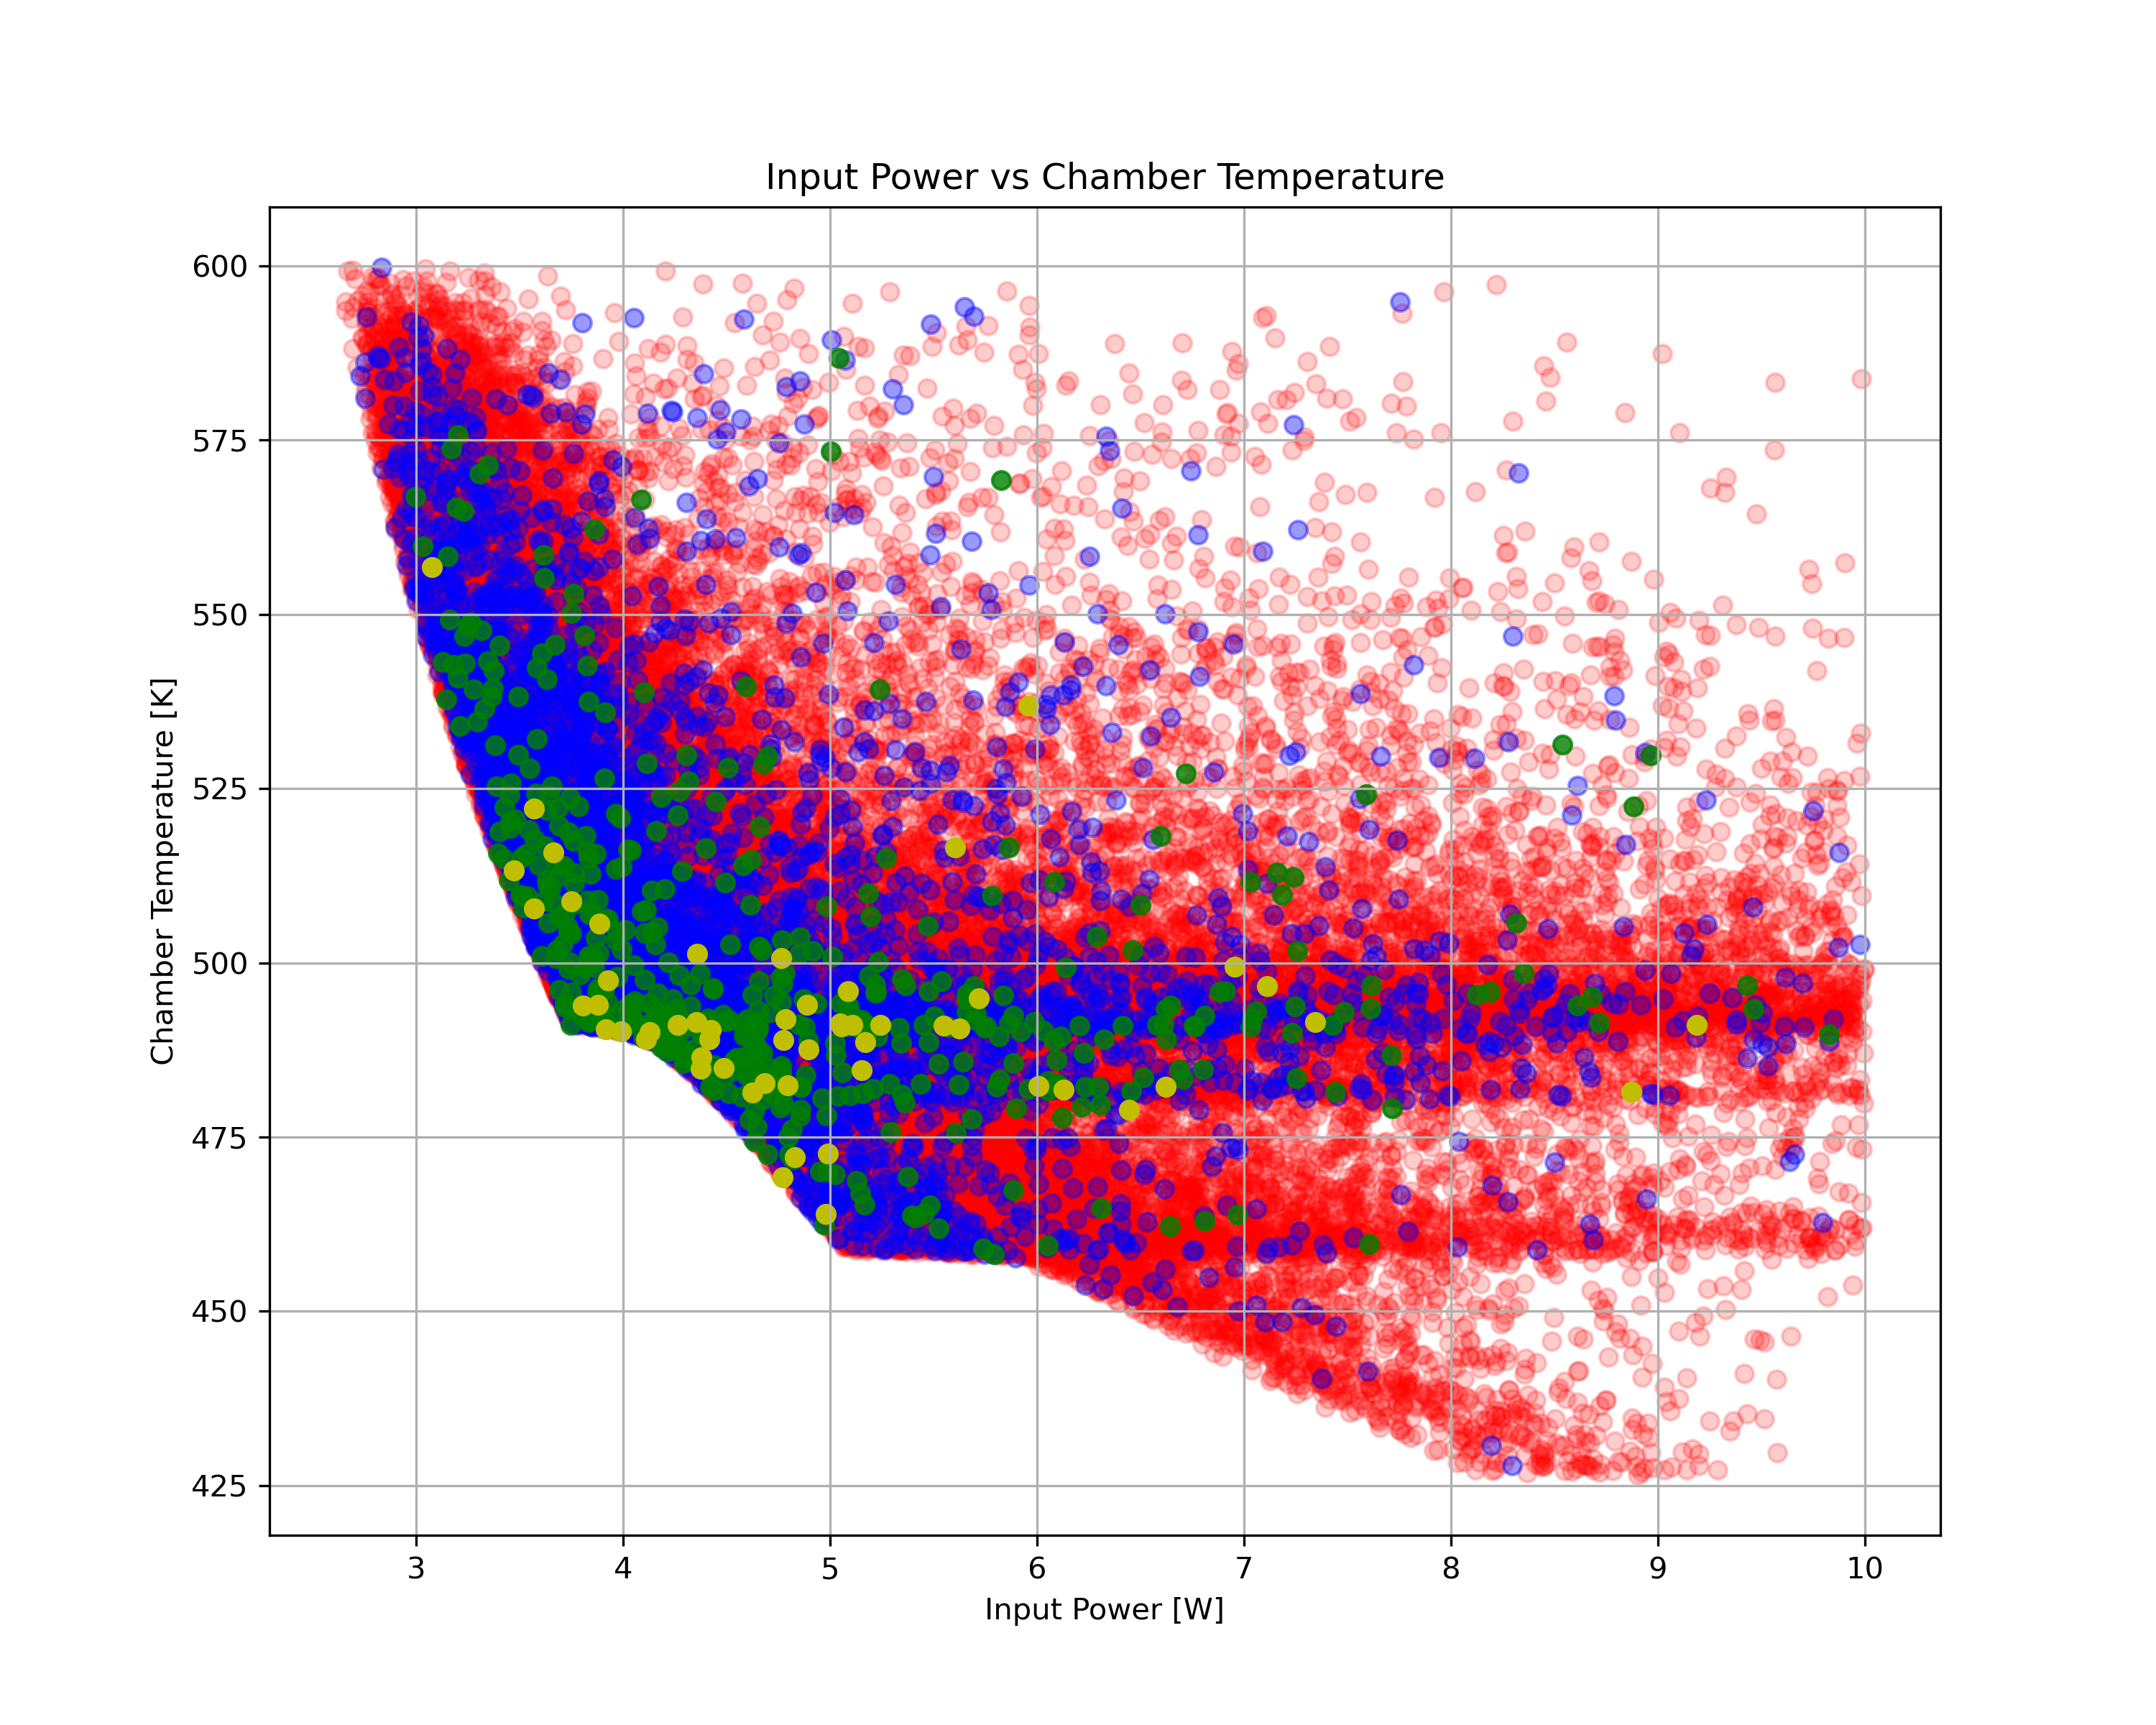
\includegraphics[width=\linewidth]{images/input_power_chamber_temperature.png}
  \captionof{figure}{Input Power vs. Chamber Temperature}
  \label{fig:power_chamber_temp}
\end{minipage}

\begin{minipage}{\linewidth}
  \centering
  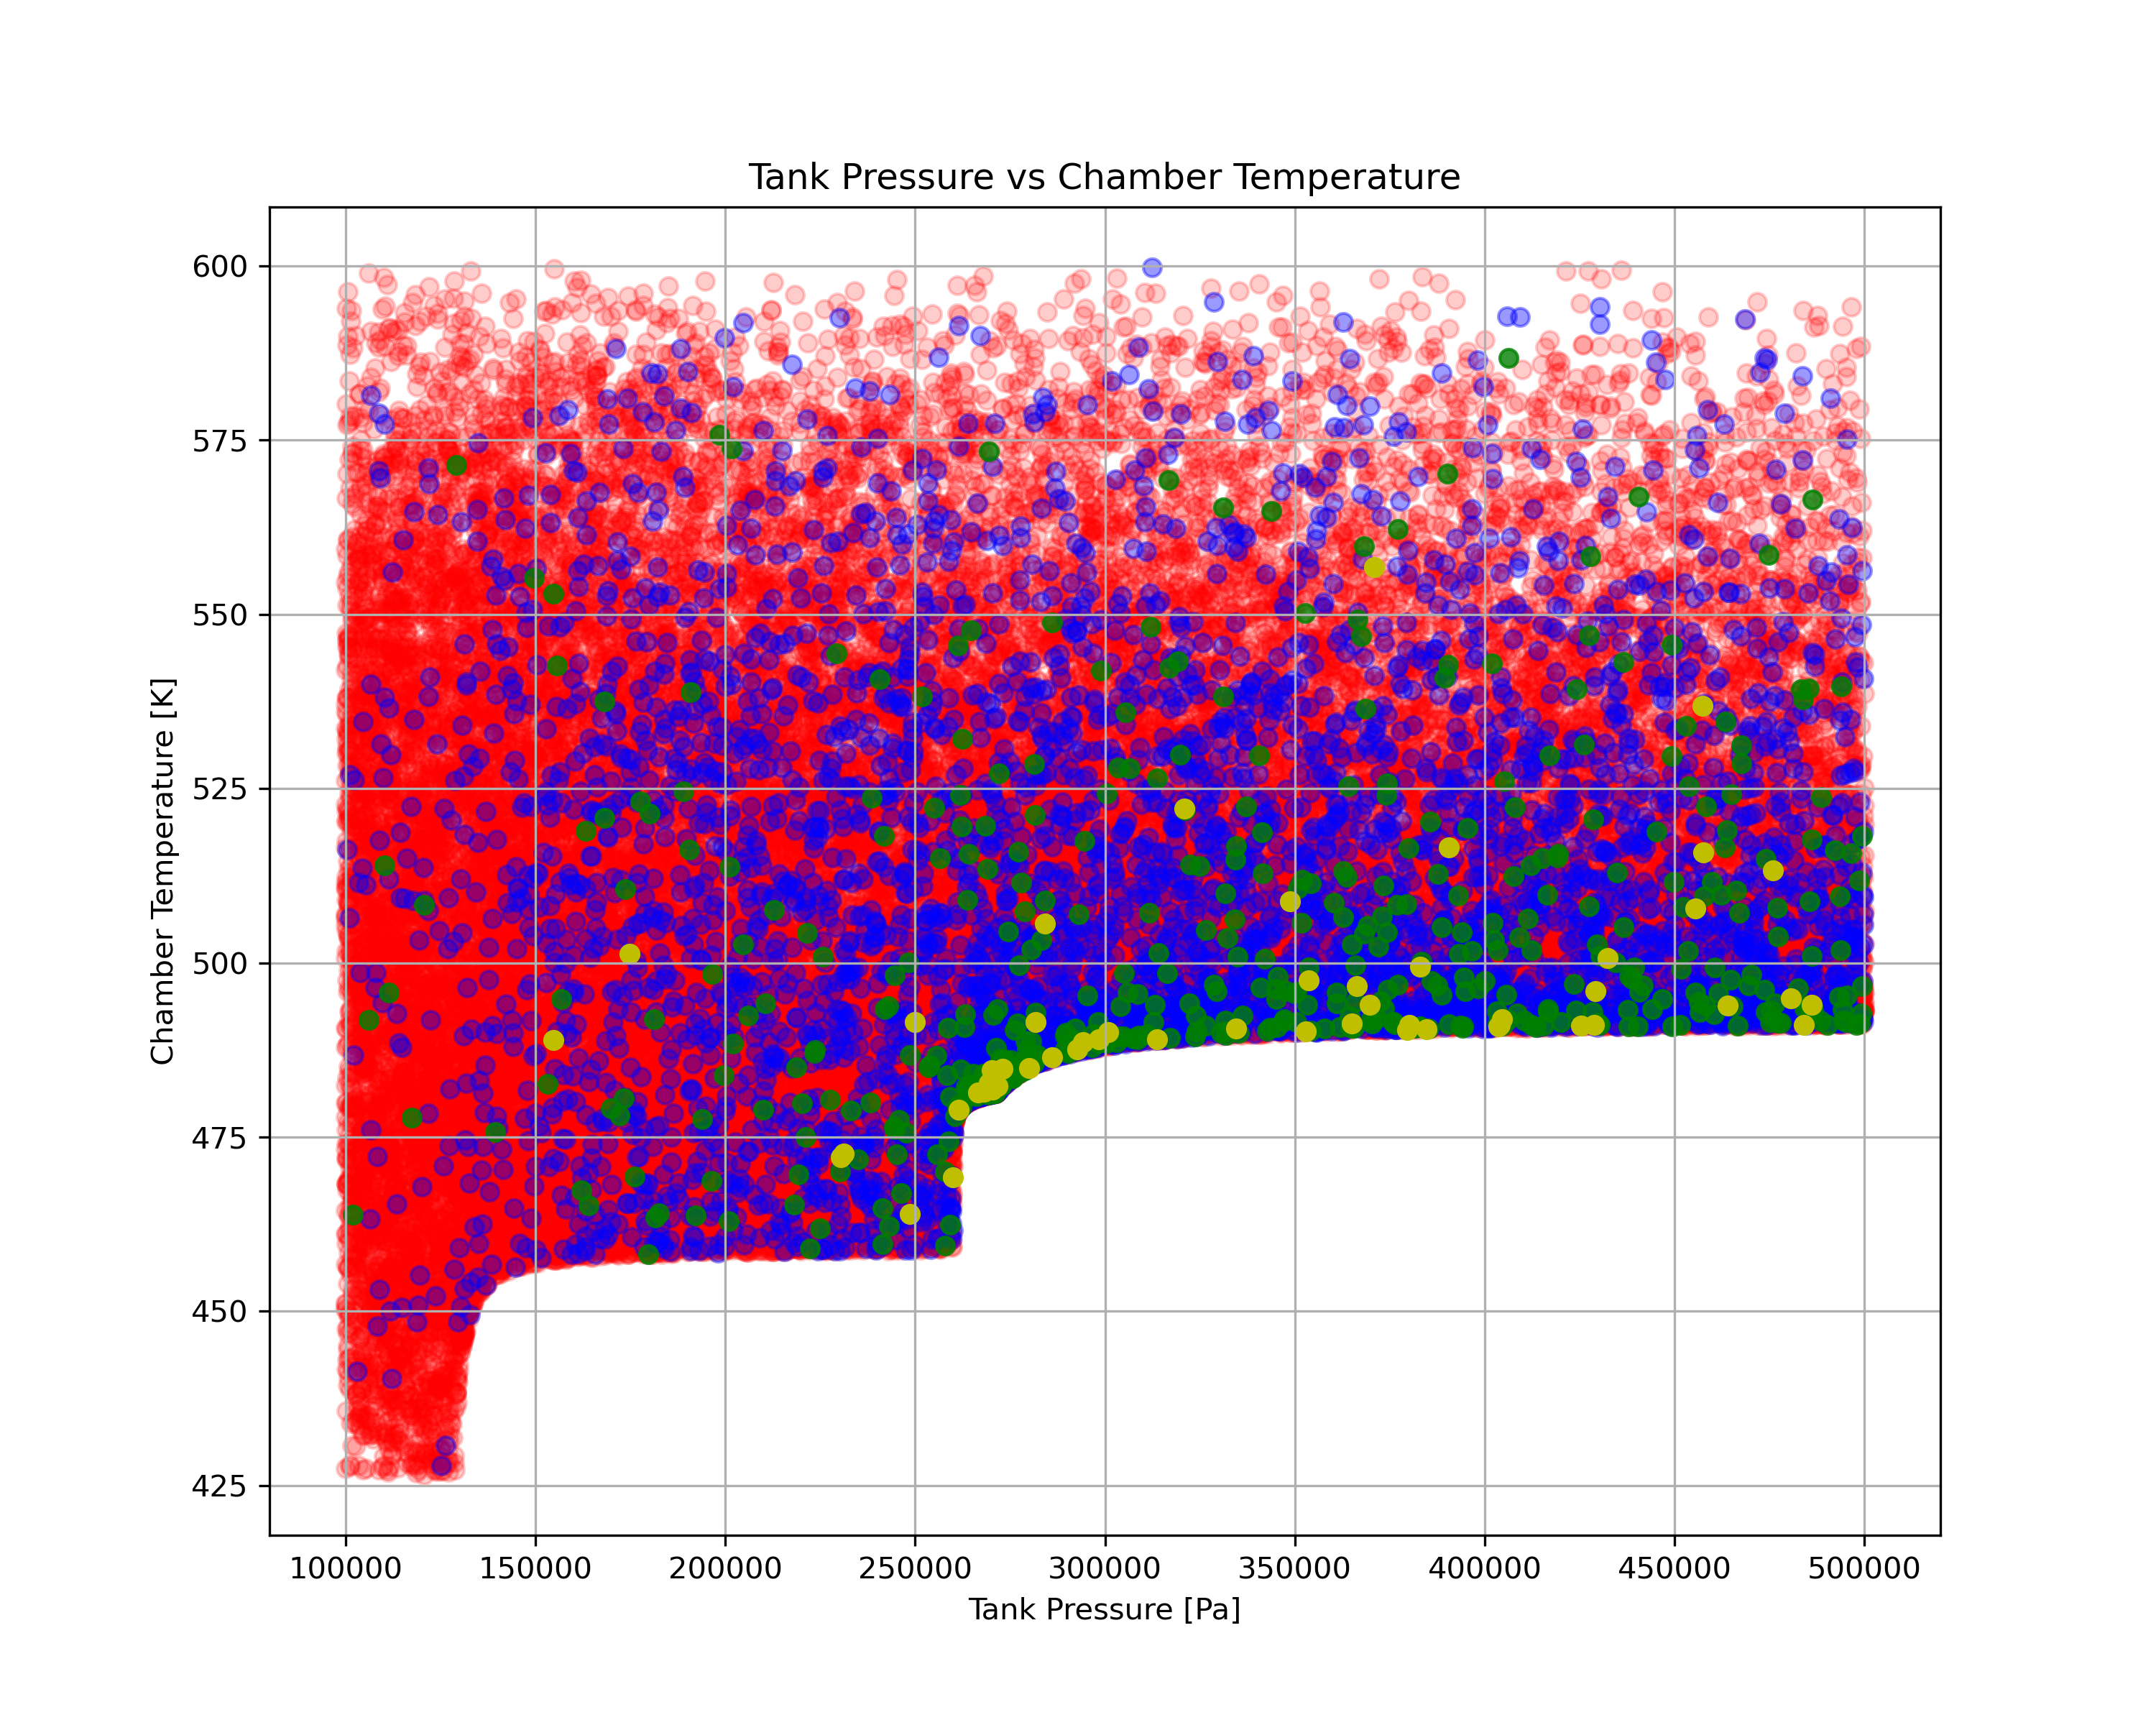
\includegraphics[width=\linewidth]{images/tank_pressure_chamber_temperature.png}
  \captionof{figure}{Tank Pressure vs. Chamber Temp. (new)}
  \label{fig:pressure_chamber_temp}
\end{minipage}

\textbf{Combined Eval. Par.}: The evaluation parameter is only useful insofar as it helps model priorities for specific kinds of performance, so a total decrease does not reveal much about actual performance.


\textbf{Tank Pressure}: The significantly reduced required pressure is a gain, since lower tank pressure simplifies tank design and reduces structural demands.

\textbf{Nozzle Exit and Throat Radii}: While the exit got 1.74\% larger, the throat area increased by 39\%, indicating an expansion ratio decrease from 9.66 to 5.21, or  46\%. The decreased Mach number yields, when combined with the lower chamber temperature, a decreased exit velocity and thus a lower $I_{sp}$, since the mass flow remained relatively constant. If the design were also evaluated by its specific impulse rather than just the specific impulse efficiency, the best design would likely reflect this change in priorities.

% Figures \ref{fig:expansion_ratio_score} and \ref{fig:pressure_expansion_ratio} tell an interesting story about the relationship between the expansion ratio and other performance indicators: most of the top 1\% designs cluster around an expansion ratio of 4-7, while the pressure ratio in that range is around 0.025 and largely invariant to the expansion ratio.

% The equation for true thrust may hold the answer, since the negative pressure ratio is a contributing term. However, the divergence loss $\epsilon_{\text {div }}$ is greatly increased for large exit radii, and as the momentum loss is proportional to exit velocity $\Delta F_{\text {momentum }} \ \alpha \ u_e^2$, which is largely mediated by the exit Mach number, it may make sense that larger expansion radii have worse non-ideal thrust performance.

% \begin{minipage}{\linewidth}
%       \centering
%       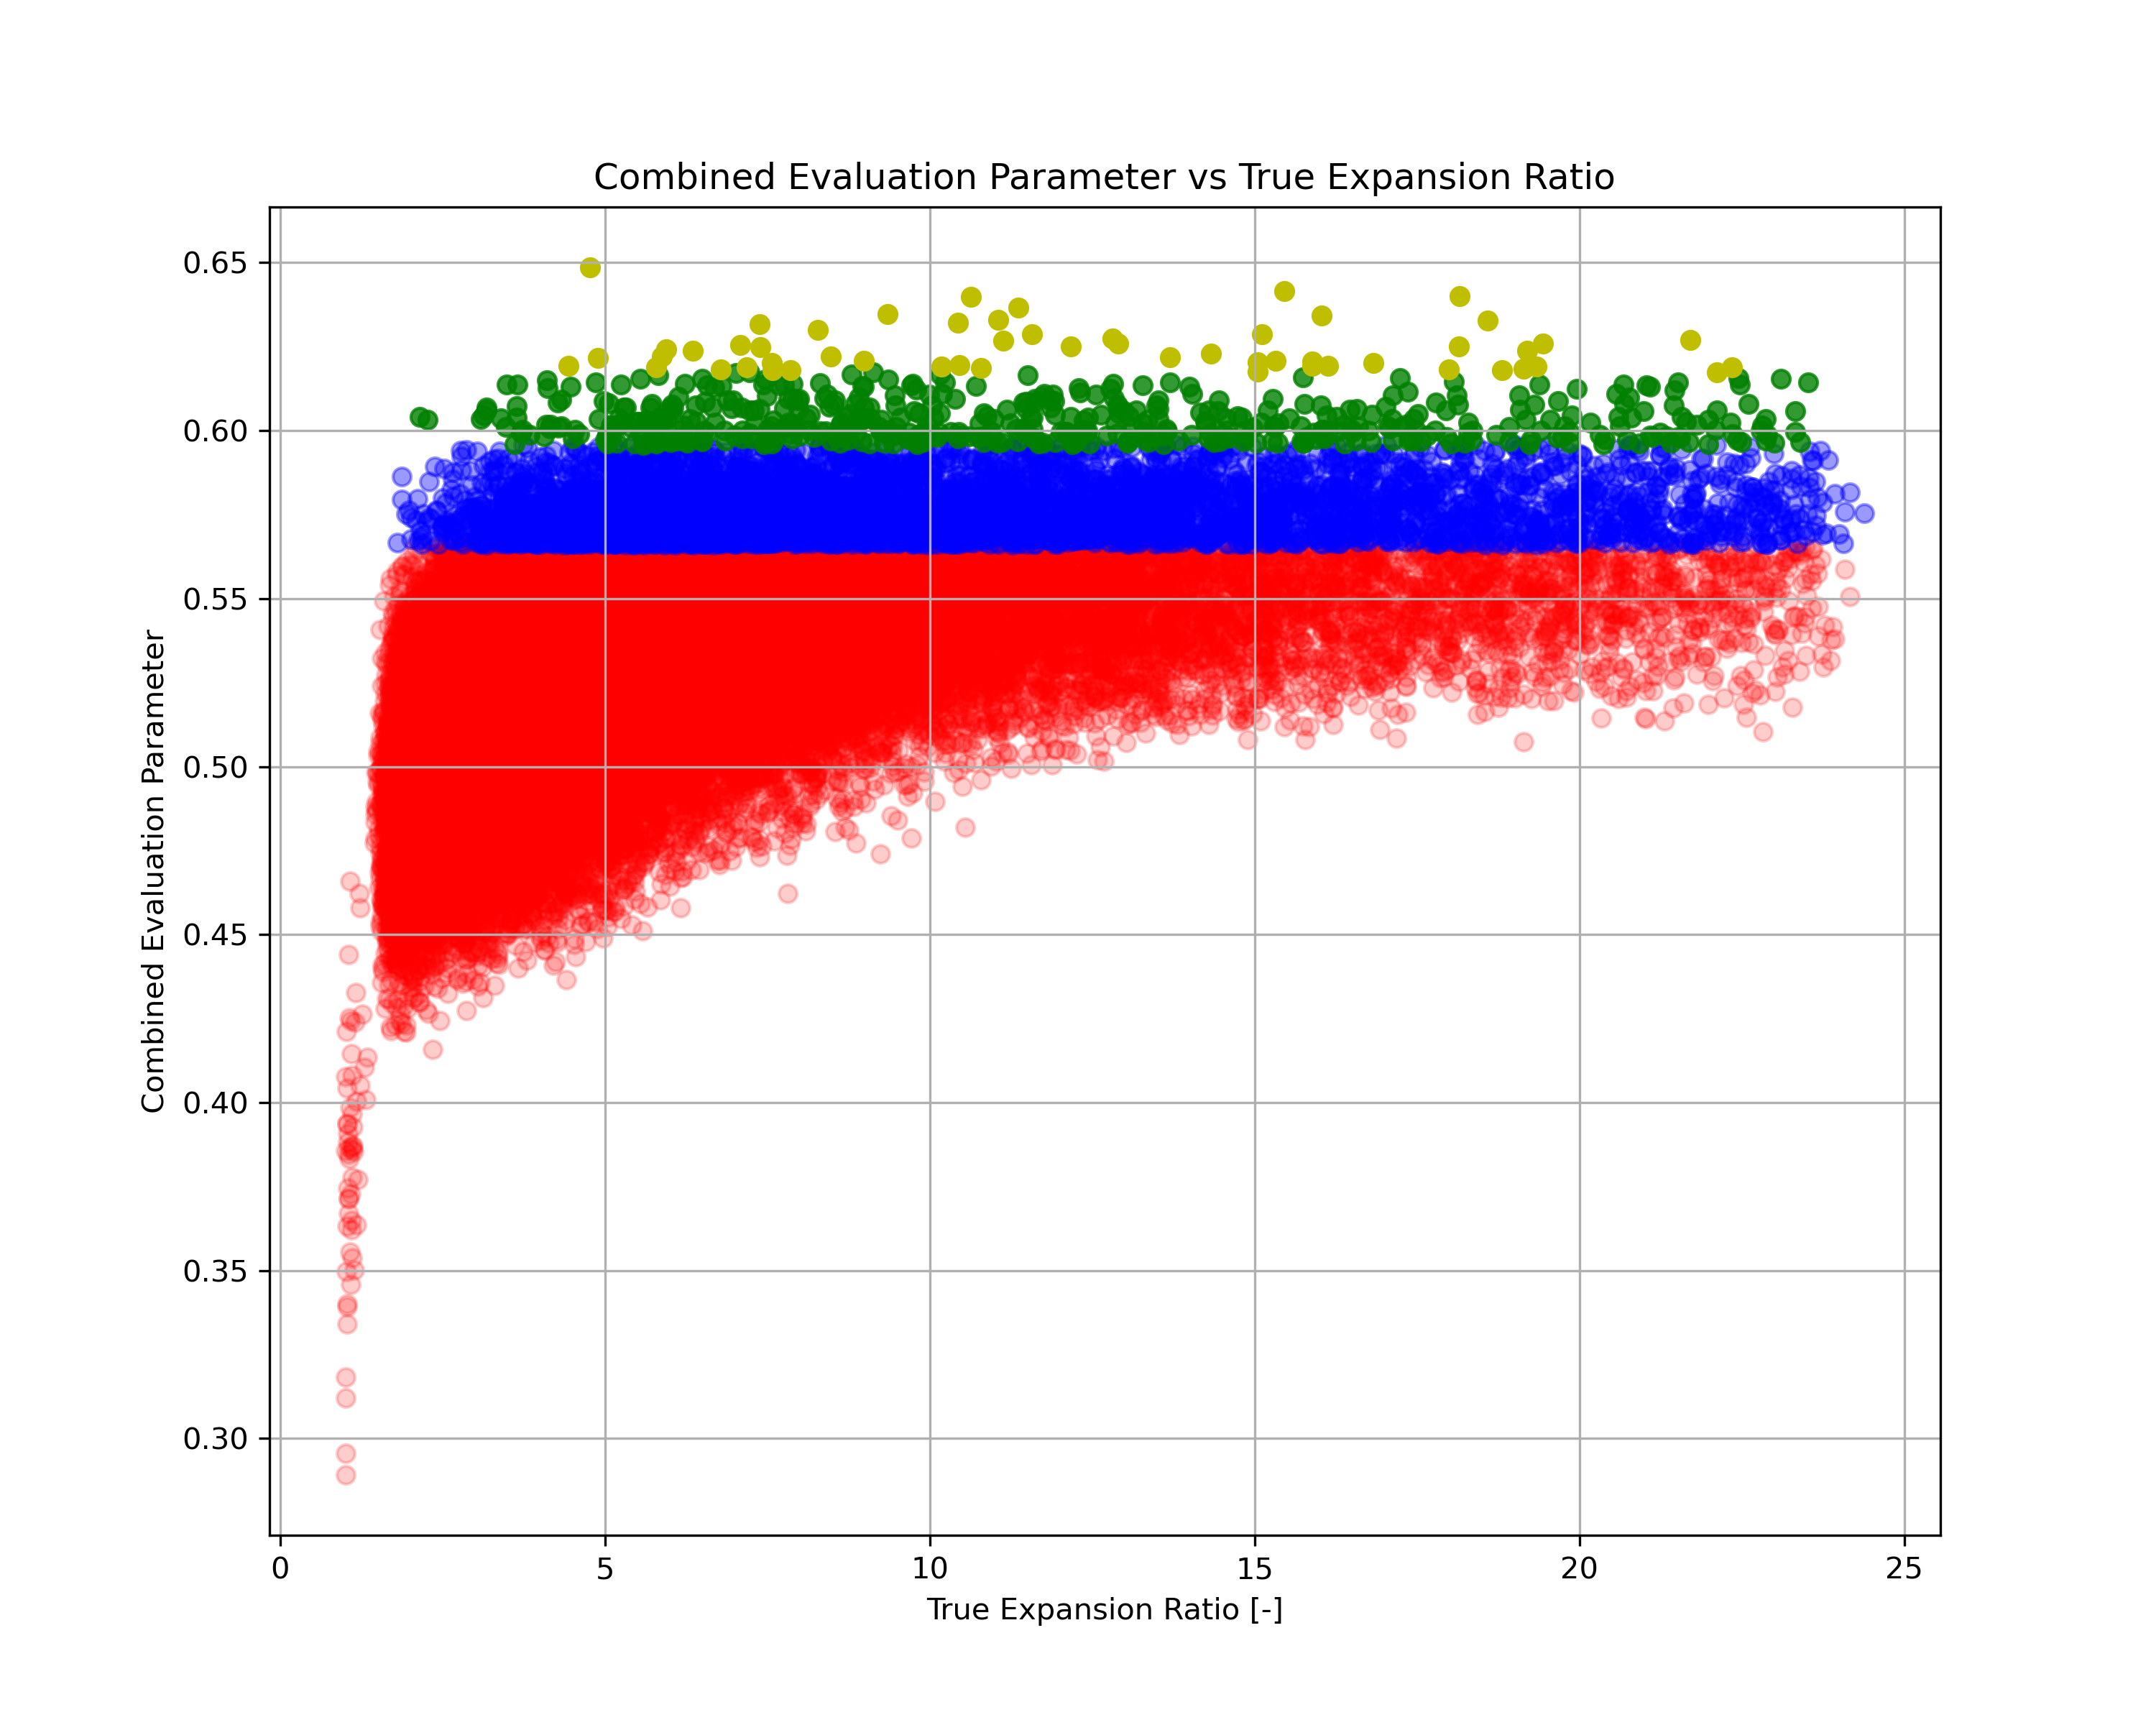
\includegraphics[width=\linewidth]{images/true_expansion_ratio_score.png}
%       \captionof{figure}{True Expansion Ratio vs. Evaluation Par.}
%       \label{fig:expansion_ratio_score}
%   \end{minipage}

%   \begin{minipage}{\linewidth}
%   \centering
%   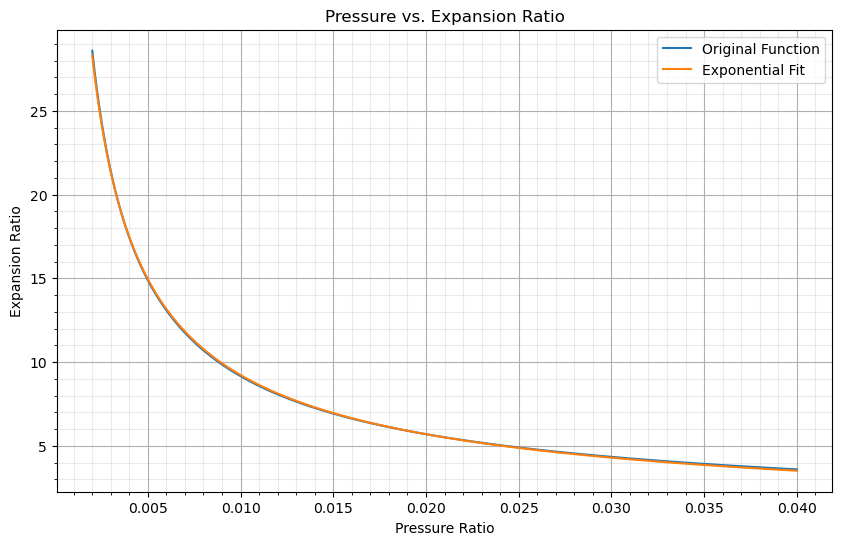
\includegraphics[width=\linewidth]{images/pressure_vs_expansion_ratio.png}
%   \captionof{figure}{Pressure Ratio vs. Expansion Ratio}
%   \label{fig:pressure_expansion_ratio}
% \end{minipage}


% \begin{align*}		    
% &F_{\text {true }}=\dot{m}_{true} \cdot \epsilon_{\text {div }} \cdot \\
% & \sqrt{2 \cdot \frac{\gamma}{\gamma-1} \cdot R_s \cdot \mathrm{T}_{\mathrm{c}} \cdot\left(1-\left(\frac{\mathrm{p}_{\mathrm{e}}}{\mathrm{p}_{\mathrm{c}}}\right)_{\text {true }}^{\frac{\gamma-1}{\gamma}}\right)}\\
% &-\Delta F_{\text {momentum }}
% \end{align*}

\textbf{Nozzle Length}: The small increase is negative, as shorter nozzles are generally more efficient. A shorter nozzle will decrease the momentum thickness and thus displacement thickness, allowing the boundary layer in the nozzle less time to grow and affect the effect exit area.

\section{Conclusion and \\ Discussion}

The model presented in this paper was an attempt to synthesize and combine existing models for more accurate VLM performance estimation, but there are are still holes in the theory. The most important problems to resolve are the very low Reynolds numbers in the heating chamber and associated Nusselt numbers which may not be physically accurate, although the limited time to complete the research precluded this being investigated further. The many assumptions underlying the theory used in this model should be investigated experimentally to be validated within an acceptable error tolerance, as much of the theory behind pressure losses due to microchannel effects was ignored to the relatively small loss compared to the operating pressure. The input ranges used for simulation were chosen in accordance with the precedent set by previous designs, but it is possible that they could be constrained for a deeper, more accurate search or expanded to include other possible designs.

Generally speaking, the utility of the work done here is to provide a modeling and optimization framework which can be modified with relative ease to include more accurate equations and still search an entire multidimensional design space effectively. That said, the algorithmic quality of the code still has significant room for improvement, since the generation of the latter 100,000 samples took nearly half an hour. Optimizations may be achieved by opting for a lower level language than Python and employing vectorized functions, better optimizer algorithms, adaptive sample generation to fully cover the design space, among other modifications. 

Concerning the choice of optimal design, the evaluation score used was very simple and could benefit from refinement. This includes investigating the correlation and higher order effects between variables that may lead to disproportionate effect on the final score, as well as reevaluating the parameters included in the scores, and their relative importance. This will depend on the goals of the designer, but using the provided codebase, they can relatively quickly optimize a design solely for size or thrust, for example.

\bibliographystyle{plain} % We choose the "plain" reference style
\bibliography{refs} % Entries are in the refs.bib file

\end{multicols}
\end{document}
